% Sumber LaTeX untuk buku ``Metode Aljabar'' dalam bahasa Tionghoa
% Hak cipta 2018  Wen-Wei Li.
% Izin diberikan untuk menyalin, menyebarluaskan, dan/atau mengubah
% dokumen ini berdasarkan ketentuan Creative Commons
% Atribusi 4.0 Internasional (CC BY 4.0)
% http://creativecommons.org/licenses/by/4.0/

% Untuk disertakan
\chapter{Teori Galois}\label{sec:Galois}
Tujuan mula-mula teori Galois ialah mempelajari penyelesaian persamaan polinomial dengan meninjau permutasi akar-akarnya. Setelah dirumuskan kembali oleh E.\ Artin dan yang lain, dalam sudut pandang modern teori Galois lebih tepat dipandang sebagai komponen inti teori medan: teori ini mempelajari ekstensi separabel dan normal (yakni ekstensi Galois) beserta automorfismenya (yang membentuk grup Galois). Hasil utamanya adalah korespondensi Galois (Teorema \ref{prop:finite-Galois-corr}, \ref{prop:infinite-Galois-corr}), yang dapat dipahami sebagai kamus penghubung sifat-sifat teori medan dan teori grup. Teori ini mempunyai tiga penerapan klasik:
\begin{compactenum}[(a)]
	\item masalah konstruksi dengan penggaris dan jangka,
	\item bukti teorema dasar aljabar melalui teori medan,
	\item kriteria keterpecahan persamaan polinomial dengan radikal.
\end{compactenum}
Untuk ketiga pokok ini sudah tersedia buku teks yang sangat baik, misalnya \cite{ZhP}. Karena itu kita hanya menyinggung (a) dan (c), sedangkan (b) ditempatkan sebagai latihan. Selain keterbatasan ruang, alasannya ialah bahwa ``bukti aljabar murni'' bagi teorema dasar aljabar merupakan cita-cita yang tidak realistis (medan $\R$ dan $\CC$ sendiri tidak mempunyai definisi yang murni aljabar); menolak alat analisis pun sukar dianggap sehat, kecuali jika hal itu menyingkap hakikat masalah atau memperluas sudut pandang. Tujuan utama bab ini ialah menyajikan pernyataan-pernyataan umum dan struktural yang diperlukan untuk studi lebih lanjut. Atas dasar itu, kriteria Galois bagi keterpecahan dengan radikal (Teorema \ref{prop:characterization-solvable-radicals}) akan diperoleh sebagai penerapan teori Kummer, dan ekstensi Galois tak hingga akan dibahas secara khusus karena diperlukan dalam praktik.

\begin{wenxintishi}
	Cara baku menangani ekstensi Galois tak hingga ialah memperkenalkan sedikit bahasa topologi, yakni topologi Krull pada grup Galois. Pembaca pemula boleh melewatinya terlebih dahulu; cukup diperhatikan bahwa hampir semua pernyataan tentang ekstensi Galois tak hingga dibuktikan dengan mereduksinya pada kasus hingga. Untuk teori Kummer, cara paling ringkas memakai kohomologi Galois $\Hm^0$, $\Hm^1$, dan dualitas Pontryagin bagi grup topologis. Demi menghindari terlalu banyak perangkat, \S\ref{sec:Kummer-theory} mengambil jalan yang agak memutar; bagaimanapun penyajiannya, inti teknis dalam penerapan tetaplah Teorema Hilbert 90.
\end{wenxintishi}

\section{Korespondensi Galois Hingga}
Ingat bahwa $\Aut_F(E)$ menyatakan grup automorfisme ekstensi medan $E|F$, sedangkan $\Aut(E)$ menyatakan grup automorfisme medan $E$. Jika medan prima $E$ ditulis $\Bbbk$, maka $\Aut(E)=\Aut_\Bbbk(E)$.

\begin{definition}\label{def:Galois-ext} \index{ekstensi medan!Galois}\index{grup Galois}\index[sym1]{Gal@$\Gal$}
	Ekstensi separabel dan normal $E|F$ disebut \emph{ekstensi Galois}. Grup Galois yang bersesuaian didefinisikan sebagai $\Gal(E|F):=\Aut_F(E)$.
	
	Kita lazim memakai sifat teori grup dari $\Gal(E|F)$ untuk menggambarkan $E|F$. Misalnya, $E|F$ disebut ekstensi abelian (atau siklik, solvabel, dan sebagainya) jika $\Gal(E|F)$ sebagai grup bersifat abelian (atau siklik, solvabel, dan sebagainya).
\end{definition}
Dengan menguraikan definisi separabilitas dan normalitas, suatu ekstensi Galois tidak lain adalah medan pemisah bagi suatu keluarga polinomial tak tereduksi tanpa akar berulang. Kita akan segera menghubungkannya dengan grup automorfisme; sebelumnya diperlukan beberapa sifat dasar ekstensi Galois.

\begin{lemma}\label{prop:Galois-properties}
	Ekstensi Galois memenuhi sifat-sifat berikut.
	\begin{enumerate}[(i)]
		\item Ekstensi $L|F$ Galois $\implies$ untuk setiap medan antara $E$, ekstensi $L|E$ tetap Galois.
		\item Misalkan $L|F$ dan $M|F$ merupakan subekstensi dari $\Omega|F$. Maka $L|F$ Galois $\implies$ $LM|M$ Galois.
		\item Dalam ekstensi tetap $\Omega|F$, kompositum dan irisan dari sebarang keluarga subekstensi Galois tetap merupakan ekstensi Galois.
	\end{enumerate}
\end{lemma}
\begin{proof}
	Gabungkan Proposisi \ref{prop:normal-ext-properties} (normalitas) dan Proposisi \ref{prop:sep-ext-dist} (separabilitas).
\end{proof}

Mulai sekarang tetapkan suatu penutup aljabar $\overline{F}|F$. Ingat bahwa setiap ekstensi normal $E|F$ dapat dibenamkan ke dalam $\overline{F}$. Setelah suatu pembenaman dipilih, Definisi--Teorema \ref{def:normal-ext} bersama Lema \ref{prop:alg-ext-endomorphism} memberikan $\Hom_F(E,\overline{F})=\Aut_F(E)$.
\begin{proposition}\label{prop:Galois-order-degree}
	Untuk setiap ekstensi Galois hingga $E|F$ berlaku $|\Gal(E|F)|=[E:F]$.
\end{proposition}
\begin{proof}
	Pembahasan di atas memberikan $|\Hom_F(E,\overline{F})|=|\Gal(E|F)|$, sedangkan separabilitas memberikan $|\Hom_F(E,\overline{F})|=[E:F]_s=[E:F]$.
\end{proof}

Kita memperkenalkan sepasang operasi penting dalam teori Galois. Untuk sebarang ekstensi $E|F$:
\begin{enumerate}
	\item bagi subgrup $H$ dari $\Aut_F(E)$, definisikan \emph{medan tetap}-nya sebagai $E^H:=\{x\in E:\forall\sigma\in H,\;\sigma(x)=x\}$; jelas $E^H|F$ merupakan subekstensi dari $E|F$;\index[sym1]{$E^H$}
	\item bagi subekstensi $K|F$ dari $E|F$ (atau singkatnya medan antara), definisikan subgrup $\Aut_K(E)$ dari $\Aut_F(E)$.
\end{enumerate}
Dengan demikian diperoleh
\begin{equation}\label{eqn:Galois-corr}\begin{tikzcd}[row sep=small]
	\left\{ \text{medan antara}\; K  \right\} \arrow[yshift=0.5ex, r] & \left\{\text{subgrup}\; H \subset \Aut_F(E) \right\} \arrow[yshift=-0.5ex, l] \\
	K|F \arrow[r, mapsto] & \Aut_K(E) \\
	E^H|F & H \arrow[l, mapsto]
\end{tikzcd}\end{equation}
Pasangan peta ini mempunyai sifat-sifat elementer berikut.
\begin{enumerate}
	\item Kedua sisi di atas merupakan himpunan terurut parsial terhadap $\subset$, dan kedua peta membalik urutan:
		\[ H_1 \subset H_2 \implies E^{H_1} \supset E^{H_2}, \quad K_1 \subset K_2 \implies \Aut_{K_1}(E) \supset \Aut_{K_2}(E). \]
	\item Berlaku $K\subset E^{\Aut_K(E)}$ dan $H\subset\Aut_{E^H}(E)$.
	\item Grup $\Aut_F(E)$ beraksi dari kiri pada kedua sisi: pada medan antara melalui $(\sigma,K)\mapsto\sigma(K)$, dan pada subgrup melalui konjugasi $(\sigma,H)\mapsto\sigma H\sigma^{-1}$, dengan $\sigma\in\Aut_F(E)$.
	\item Untuk aksi $\sigma\in\Aut_F(E)$ tersebut berlaku hubungan ``pemindahan struktur'' berikut:
		\[ \Aut_{\sigma(K)}(E) = \sigma \Aut_K(E) \sigma^{-1}, \quad E^{\sigma H \sigma^{-1}} = \sigma(E^H). \]
\end{enumerate}

\begin{lemma}\label{prop:invariant-field-is-F}
	Bagi ekstensi Galois $E|F$ berlaku $E^{\Gal(E|F)}=F$, dan peta $K\mapsto\Aut_K(E)=\Gal(E|K)$ bersifat injektif.
\end{lemma}
\begin{proof}
	Inti bagian pertama ialah membuktikan $E^{\Gal(E|F)}\subset F$. Ambil $x\in E^{\Gal(E|F)}$, dan seperti biasa tulis polinomial minimalnya sebagai $P_x\in F[X]$. Normalitas memastikan bahwa $P_x$ terurai menjadi faktor-faktor linear di $E$, sedangkan separabilitas memastikan tidak ada akar berulang. Untuk setiap akar $y\in E$, terdapat pembenaman-$F$ $\iota:F(x)\to F(y)\subset E$ yang memetakan $x$ ke $y$. Proposisi \ref{prop:normal-ext-prolongation} memperluas $\iota$ menjadi $\sigma\in\Gal(E|F)$. Menurut hipotesis, $y=\sigma(x)=x$; jadi $\deg P_x=1$ dan $x\in F$.
	
	Karena $E|K$ juga Galois, bagian pertama memberikan $E^{\Gal(E|K)}=K$. Maka $K\mapsto\Gal(E|K)$ injektif.
\end{proof}

\begin{lemma}\label{prop:invariant-field-transport}
	Dengan notasi di atas, untuk setiap medan antara $K$ dan $\sigma\in\Gal(E|F)$ berlaku
	\[ \Gal(E|\sigma K) = \sigma \Gal(E|K) \sigma^{-1}, \]
	dan $\Gal(E|K)\lhd\Gal(E|F)$ jika dan hanya jika $K|F$ merupakan ekstensi Galois.
\end{lemma}
\begin{proof}
	Persamaan yang ditampilkan telah diamati sebelumnya. Karena $K\mapsto\Gal(E|K)$ injektif dan $\sigma$ sebarang, $\Gal(E|K)\lhd\Gal(E|F)$ jika dan hanya jika $\sigma(K)=K$ untuk setiap $\sigma$; ini ekuivalen dengan normalitas $K|F$ (Korolari \ref{prop:normal-subext}). Di pihak lain, subekstensi dari ekstensi separabel tetap separabel (Proposisi \ref{prop:sep-ext-dist}), sehingga syarat tersebut ekuivalen pula dengan $K|F$ Galois.
\end{proof}

Jika $[E:F]$ tak hingga, peta dalam Lema \ref{prop:invariant-field-is-F} tidak surjektif. Bagian ini bertujuan membuktikan bahwa \eqref{eqn:Galois-corr} benar-benar bijektif untuk ekstensi Galois hingga.
\begin{lemma}[E.\ Artin]\label{prop:invariant-field-Galois-finite}
	Misalkan $E$ suatu medan dan $H$ subgrup hingga dari $\Aut(E)$. Maka $E|E^H$ merupakan ekstensi Galois dan $\Gal(E|E^H)=H$.
\end{lemma}
\begin{proof}
	Pertama-tama kita buktikan bahwa $E|E^H$ Galois. Biarkan $\Aut(E)$ beraksi pada gelanggang polinomial $E[X]$ melalui koefisien; dengan demikian $\sigma(f_1\pm f_2)=\sigma(f_1)\pm\sigma(f_2)$, $\sigma(f_1f_2)=\sigma(f_1)\sigma(f_2)$, dan seterusnya. Ambil $x\in E$, lalu tetapkan $\mathcal{O}:=\{\tau(x):\tau\in H\}$ dan $Q_x:=\prod_{y\in\mathcal{O}}(X-y)$. Maka $Q_x\in E[X]^H=E^H[X]$ dan $Q_x(x)=0$. Karena $Q_x$ terurai menjadi faktor linear di $E$ dan tidak mempunyai akar berulang, $E|E^H$ merupakan ekstensi separabel dan normal. Perhatikan pula bahwa $\deg Q_x=|\mathcal{O}|\leq|H|$.
	
	Kunci bagian yang tersisa ialah menetapkan pertidaksamaan
	\begin{equation}\label{eqn:Artin-ineq}
		\left[ E:E^H \right] \leq |H|.
	\end{equation}
	Argumen di atas menunjukkan $x\in E\implies[E^H(x):E^H]\leq|H|$. Pilih $x\in E$ agar $[E^H(x):E^H]$ sebesar mungkin. Jika $E=E^H(x)$, kita memperoleh \eqref{eqn:Artin-ineq}. Jika tidak, ambil $y\in E\smallsetminus E^H(x)$; maka
	\[ E^H(x,y) \supsetneq E^H(x) \supset E^H. \]
	Karena $E|E^H$ separabel, Teorema \ref{prop:prim-element-separable} memungkinkan kita menulis $E^H(x,y)$ dalam bentuk $E^H(z)$ untuk suatu $z \in E$. Akibatnya $[E^H(z):E^H] > [E^H(x):E^H]$, bertentangan dengan pilihan $x$.
	
	Ingat $H\subset\Gal(E|E^H)$. Hasil-hasil di atas menunjukkan bahwa $E|E^H$ hingga, dan
	\[ \left[ E:E^H \right] \stackrel{\eqref{eqn:Artin-ineq}}{\leq} |H| \leq |\Gal(E|E^H)| \xlongequal{\because\; \text{Proposisi \ref{prop:Galois-order-degree}}} \left[ E:E^H \right]. \]
	Jadi semua pertidaksamaan adalah kesamaan, dan $H=\Gal(E|E^H)$.
\end{proof}

\begin{theorem}[Korespondensi Galois hingga]\label{prop:finite-Galois-corr}\index{korespondensi Galois@korespondensi Galois (Galois correspondence)}
	Misalkan $E|F$ ekstensi Galois hingga. Maka \eqref{eqn:Galois-corr} memberikan bijeksi-bijeksi yang saling invers
	\[ \begin{tikzcd}[row sep=small]
	\left\{ \text{medan antara}\; K  \right\} \arrow[yshift=0.5ex, r] & \left\{\text{subgrup}\; H \subset \Gal(E|F) \right\} \arrow[yshift=-0.5ex, l] \\
		K|F \arrow[r, mapsto] & \Gal(E|K) \\
		E^H|F & H \arrow[l, mapsto]
	\end{tikzcd}\]
	dan memenuhi sifat-sifat berikut:
	\begin{enumerate}[(i)]
		\item Membalik urutan: $H_1\subset H_2\iff E^{H_1}\supset E^{H_2}$ dan $K_1\subset K_2\iff\Aut_{K_1}(E)\supset\Aut_{K_2}(E)$.
		\item Bijeksi tersebut ekuivarian terhadap aksi kiri $\Gal(E|F)$ pada kedua sisi, dan memberikan korespondensi satu-satu antara subgrup normal $H\lhd\Gal(E|F)$ dan subekstensi Galois $K|F$.
		\item Untuk setiap medan antara $K$ terdapat bijeksi
			\begin{align*}
				\Gal(E|F)\big/ \Gal(E|K) & \longrightiso \Hom_F(K, E) \\
				\sigma \cdot \Gal(E|K) & \longmapsto \sigma|_K,
			\end{align*}
			dan $(\Gal(E|F):\Gal(E|K))=[K:F]$. Jika $K|F$ Galois, peta di atas menginduksi isomorfisme grup
				\[ \Gal(E|F)\big/ \Gal(E|K) \rightiso \Gal(K|F). \]
	\end{enumerate}
	Khususnya, $|\Gal(E|F)|=[E:F]$.
\end{theorem}
\begin{proof}
	Dengan menggabungkan Lema \ref{prop:invariant-field-is-F} dan \ref{prop:invariant-field-Galois-finite}, terlihat bahwa \eqref{eqn:Galois-corr} memang memberikan bijeksi-bijeksi yang saling invers. Sifat pembalikan urutan dalam (i) telah diketahui, sedangkan (ii) merupakan perumusan ulang Lema \ref{prop:invariant-field-transport}.
	
	Untuk (iii), restriksi $\sigma,\sigma'\in\Gal(E|F)$ pada $K$ sama jika dan hanya jika $\sigma^{-1}\sigma'|_K=\identity_K$; jadi terdapat injeksi $\Gal(E|F)/\Gal(E|K)\to\Hom_F(K,E)$. Di pihak lain, setiap elemen $\Hom_F(K,E)$ dapat diperluas menjadi elemen $\Gal(E|F)$ (Proposisi \ref{prop:normal-ext-prolongation}), sehingga peta tersebut bijektif.
	
	Untuk membuktikan bahwa kardinalitas $\Hom_F(K,E)$ adalah $[K:F]=[K:F]_s$, tetapkan suatu penutup aljabar $\overline{F}|E$ dan perhatikan $\Hom_F(K,E)=\Hom_F(K,\overline{F})$. Ini merupakan penerapan langsung Korolari \ref{prop:normal-subext} pada menara ekstensi $\overline{F}|E|K|F$.

	Jika $K|F$ Galois, Korolari \ref{prop:normal-subext}, diterapkan pada menara $E|K|K|F$, memberikan $\Hom_F(K,E)=\Hom_F(K,K)=\Gal(K|F)$; dengan demikian $\sigma\mapsto\sigma|_K$ adalah homomorfisme grup. Selesai.
\end{proof}

Korespondensi Galois hingga sesungguhnya merupakan landasan kasus tak hingga. Bukti umum dan sifat-sifat lanjutannya disajikan dalam \S\ref{sec:inf-Galois}.

\begin{example}
	Tinjau kembali medan pemisah $\Q(\sqrt[3]{2},\omega)$ dari $X^3-2\in\Q[X]$ pada Contoh \ref{eg:x3-2-splitting}, dan perhatikan bahwa polinomial minimal $\omega$ di atas $\Q$ adalah $X^2+X+1$. Diagram medannya ialah:
	\[\begin{tikzcd}[column sep=small]
		{} & \Q(\sqrt[3]{2}, \omega) \arrow[dash, d, "\text{Galois}"] \arrow[dash, ld, "\text{Galois}"'] \\
		\Q(\sqrt[3]{2}) \arrow[dash, rd, "\text{derajat} = 3"'] & \Q(\omega) \arrow[dash, d, "{\text{Galois},\; \text{derajat} = 2}"] \\
		& \Q
	\end{tikzcd}\]
	Karena $[\Q(\sqrt[3]{2}, \omega): \Q(\omega)] \leq 3$, sedangkan $2 = [\Q(\omega) : \Q]$ dan $3 = [\Q(\sqrt[3]{2}) : \Q]$ keduanya membagi $[\Q(\sqrt[3]{2}, \omega): \Q]$, satu-satunya kemungkinan ialah $[\Q(\sqrt[3]{2}, \omega): \Q] = 6$. Jadi $G := \Gal(\Q(\sqrt[3]{2},\omega)|\Q)$ berorde $6$. Setiap $\sigma \in G$ bertindak melalui $\omega \mapsto \omega^{\pm 1}$ dan $\sqrt[3]{2} \mapsto \omega^k \sqrt[3]{2}$ ($k=0,1,2$), dan $\sigma$ sepenuhnya ditentukan oleh $(\pm, k)$. Ada paling banyak $6$ pilihan, sehingga setiap pasangan $(\pm,k)$ direalisasikan dalam $G$.

	Secara umum, grup Galois dari medan pemisah suatu polinomial separabel dapat dibenamkan sebagai subgrup grup simetris pada himpunan akarnya. Karena $|G|=6=3!$, sekarang kita dapat mengidentifikasi $G$ dengan grup simetris $\mathfrak{S}_3$ pada himpunan akar $\{\sqrt[3]{2},\omega\sqrt[3]{2},\omega^2\sqrt[3]{2}\}$. Dengan mendaftarkan subgrup dan meninjau elemen-elemen yang ditetapkannya, Teorema \ref{prop:finite-Galois-corr} memberikan korespondensi pembalik urutan berikut:
	\[\begin{tikzpicture}
		[baseline = (current bounding box.center),
			every node/.style={ },
			every edge/.style={draw},
			normaledge/.style={ sloped, edge node={node[fill=white, outer sep=0.2mm, inner sep=0mm] {$\lhd$}} }
		]
		\begin{scope}
			\node (G) at (0, 3) {$G$};
			\node (A) at (-1, 2) {$\mathfrak{A}_3$};
			\node (H1) at (-2,1.5) {$\lrangle{(1 2)}$};
			\node (H2) [right=1cm of H1] {$\lrangle{(2 3)}$};
			\node (H3) [right=0.5cm of H2] {$\lrangle{(1 3)}$};
			\node (E) at (0, 0) {$\{1\}$};
		\end{scope}
		\draw (G) edge[normaledge] (A);
		\draw (G) edge[bend right=30] (H1);  \draw (G) edge (H2);  \draw (G) edge[sloped, edge label={$\supset$}] (H3);
		\foreach \x in {A, H1, H2, H3}
			\draw (\x) edge (E);
	\end{tikzpicture} \;
	\begin{tikzpicture}[baseline= (current bounding box.center)]
		\draw[thick, dashed] (0, 1.7) -- (0, -1.7);
		\node[double arrow, draw, fill=white] at (0,0) {\scriptsize $H \leftrightarrow E^H$};
	\end{tikzpicture} \; \begin{tikzpicture}
		[baseline = (current bounding box.center),
			every node/.style={ },
			every edge/.style={draw},
			normaledge/.style={edge node={node[fill=white, outer sep=0.2mm, inner sep=0mm] {\scriptsize$\text{Galois}$}} }
		]
		\begin{scope}
			\node (FG) at (0,3) {$\Q$};
			\node (FA) at (-1, 2) {$\Q(\omega)$};
			\node (FH1) at (-2, 1.5) {$\Q(\omega^2 \sqrt[3]{2})$};
			\node (FH2) [right=0.7cm of FH1] {$\Q(\sqrt[3]{2})$};
			\node (FH3) [right=0.3cm of FH2] {$\Q(\omega\sqrt[3]{2})$};
			\node (FE) at (0,0) {$\Q(\omega, \sqrt[3]{2})$};
			\node (extra) [left=0.3cm of FE] {$E$};
			\draw (FE) edge[draw=none, edge node={node {$:=$}}] (extra);
		\end{scope}
		\draw (FG) edge[normaledge] (FA);
		\draw (FG) edge[bend right=30] (FH1);  \draw (FG) edge (FH2);  \draw (FG) edge[sloped, edge label={$\subset$}] (FH3);
		\foreach \x in {A, H1, H2, H3}
		\draw (F\x) edge (FE);
	\end{tikzpicture}\]
	Subgrup dan medan antara yang bersesuaian ditempatkan pada posisi yang sama, sedangkan garis menyatakan relasi inklusi; arah inklusi pada kedua sisi saling terbalik. Ketiga medan antara $\Q(\omega^k\sqrt[3]{2})$ ($k=0,1,2$) saling konjugat, sebagaimana jelas dari sisi teori grup.
\end{example}

\section{Korespondensi Galois Tak Hingga}\label{sec:inf-Galois}
Ketika mempelajari grup Galois suatu ekstensi Galois tak hingga, bahasa grup topologis (Definisi \ref{def:topological-group} dan pembahasan sesudahnya) sangat berguna.
\begin{definition}[Topologi Krull]\label{def:Krull-topology} \index{topologi Krull}
	Untuk ekstensi Galois $E|F$, berikan pada $\Gal(E|F)$ topologi yang mempunyai, pada setiap elemen $\sigma$, basis lingkungan
	\[ \sigma\Gal(E|K), \quad K|F: \;\text{subekstensi Galois hingga}. \]
	Topologi ini disebut \emph{topologi Krull} pada $\Gal(E|F)$.
\end{definition}

\begin{itemize}
	\item Secara intuitif, topologi Krull mengatakan: ``Jika terdapat subekstensi Galois hingga yang cukup besar $K|F$ dengan $\sigma|_K=\tau|_K$, maka $\sigma$ cukup dekat dengan $\tau$.''
	\item Karena $\Gal(E|K)$ subgrup normal (Lema \ref{prop:invariant-field-transport}), definisi tersebut dapat pula dirumuskan dengan $\Gal(E|K)\sigma$.
	\item Basis lingkungan harus tertutup terhadap irisan hingga. Hal ini dijamin oleh $\Gal(E|K)\cap\Gal(E|K')=\Gal(E|KK')$, sebab Lema \ref{prop:Galois-properties} menyatakan bahwa $KK'|F$ tetap merupakan ekstensi Galois hingga.
	\item Bagi setiap subekstensi hingga $L|F$, ambil penutupan normal dari $L$ di dalam $E$, yakni $L' \supset L$ (Definisi \ref{def:normal-closure}); $L'|F$ tetap hingga. Karena $\Gal(E|L') \subset \Gal(E|L)$, basis lingkungan dapat pula diambil berbentuk $\sigma \Gal(E|L)$, dengan $L|F$ menjelajahi semua subekstensi hingga.
	\item Dari definisi topologi Krull jelas bahwa peta invers kontinu: peta ini membawa lingkungan $\sigma\Gal(E|K)$ ke $\Gal(E|K)\sigma^{-1}=\sigma^{-1}\Gal(E|K)$. Demikian pula, perkalian membawa $\sigma\Gal(E|K)\times\tau\Gal(E|K)$ ke $\sigma\tau\Gal(E|K)$, sehingga juga kontinu. Jadi $\Gal(E|F)$ memang grup topologis.
\end{itemize}

\begin{lemma}\label{prop:infinite-Galois-profinite}
	Untuk setiap ekstensi Galois $E|F$, grup topologis $\Gal(E|F)$ merupakan grup profinit dalam arti Definisi \ref{def:profinite-group}. Lebih tepatnya, terdapat isomorfisme alami grup topologis
	\[ \Gal(E|F) \rightiso \varprojlim_{\substack{K|F: \;\text{hingga} \\ \mathrm{Galois} \;\text{subekstensi}}} \Gal(K|F). \]
\end{lemma}
Dalam bukti kita akan meninjau kembali struktur topologi limit $\varprojlim_K\Gal(K|F)$.
\begin{proof}	
	Ingat Proposisi \ref{prop:alg-ext-dist}: $E|F$ adalah gabungan subekstensi hingga $L|F$. Dengan mengganti $L$ oleh penutupan normalnya $K$, kita bahkan dapat menyatakan $E|F$ sebagai gabungan subekstensi Galois hingga $K|F$. Sifat ekstensi normal dan Lema \ref{prop:alg-ext-endomorphism} menunjukkan bahwa peta restriksi $\sigma\mapsto\sigma|_K$ memberikan homomorfisme $\Gal(E|F)\to\Gal(K|F)$. Jadi pemberian $\sigma\in\Gal(E|F)$ ekuivalen dengan pemberian keluarga $\sigma_K\in\Gal(K|F)$ yang memenuhi kompatibilitas $K'\supset K\implies\sigma_{K'}|_K=\sigma_K$; dalam bahasa limit invers, ini merupakan isomorfisme grup
	\begin{align*}
		\Gal(E|F) & \longrightiso \varprojlim_{\substack{K|F: \;\text{hingga} \\ \mathrm{Galois} \;\text{subekstensi}}} \Gal(K|F) \\
		\sigma & \longmapsto (\sigma|_K)_K
	\end{align*}
	Homomorfisme transisi dalam limit ialah peta restriksi $\Gal(K'|F)\to\Gal(K|F)$ untuk $K'\supset K$. Invers isomorfisme tersebut memetakan $(\sigma_K)_K$ ke $x\mapsto\sigma_K(x)$, dengan $K|F$ sebarang subekstensi Galois hingga yang memuat $x\in E$. Benamkan ruas kanan isomorfisme ke dalam ruang produk $\prod_K\Gal(K|F)$ dan berikan topologi diskret pada setiap $\Gal(K|F)$; ruas kanan itu tepat merupakan grup profinit dari Definisi \ref{def:profinite-group}. Di pihak lain, Lema \ref{prop:completion-compactness} telah menggambarkan basis lingkungan di $1$ bagi grup profinit. Untuk ruas kanan, basis tersebut ialah
	\[ U_L := \Ker\left[ p_L: \varprojlim_K \Gal(K|F) \longrightarrow \Gal(L|F) \right]. \]
	Tidak perlu mengambil irisan hingga lagi, sebab $U_L\cap U_M=U_{LM}$. Selain itu, melalui isomorfisme, $U_L$ bersesuaian dengan $\Gal(E|L)=\{\sigma\in\Gal(E|F):\sigma|_L=\identity_L\}$. Karena basis lingkungan elemen identitas menentukan topologi grup, $\Gal(E|F)\rightiso\varprojlim_K\Gal(K|F)$ merupakan homeomorfisme. Selesai.
\end{proof}

\begin{lemma}\label{prop:Krull-top-properties}
	Grup topologis $G:=\Gal(E|F)$ mempunyai sifat-sifat berikut:
	\begin{enumerate}[(i)]
		\item $G$ merupakan ruang Hausdorff kompak, dan mempunyai topologi diskret jika $E|F$ hingga;
		\item untuk setiap subekstensi hingga $L|F$, subgrup $\Gal(E|L)$ terbuka;
		\item setiap subgrup terbuka $H$ juga tertutup dan memenuhi $(G:H)<\infty$;
		\item untuk setiap subekstensi $L|F$, subgrup $\Gal(E|L)$ tertutup;
		\item jika $E$ diberi topologi diskret, peta aksi $\Gal(E|F)\times E\to E$ kontinu.
	\end{enumerate}
\end{lemma}
\begin{proof}
	Teorema \ref{prop:profinite-characterization} menyatakan bahwa grup profinit selalu Hausdorff kompak, sedangkan setiap topologi Hausdorff pada himpunan hingga pasti diskret; ini membuktikan (i). Lema \ref{prop:open-closed-subgroup} langsung memberikan (iii).
	
	Untuk membuktikan (ii), perhatikan dahulu bahwa bagi setiap $x\in E$, subgrup penstabil $\Stab_G(x)=\{\sigma\in G:\sigma(x)=x\}$ terbuka. Memang, $F(x)$ termuat dalam suatu subekstensi Galois hingga $K|F$ (misalnya penutupan normalnya), sehingga $\Stab_G(x)$ memuat subgrup terbuka $\Gal(E|K)$; maka $\Stab_G(x)$ terbuka (sekali lagi memakai Lema \ref{prop:open-closed-subgroup}). Jika ekstensi hingga $L|F$ ditulis $L=F(x_1,\ldots,x_n)$, maka $\Gal(E|L)=\bigcap_{i=1}^n\Stab_G(x_i)$ juga merupakan subgrup terbuka.
	
	Untuk (iv), misalkan $L|F$ sebarang subekstensi. Maka $\Gal(E|L)=\bigcap_{x\in L}\Stab_G(x)$. Setiap $\Stab_G(x)$ terbuka sekaligus tertutup, sehingga $\Gal(E|L)$ merupakan subgrup tertutup.
	
	Terakhir, untuk (v), jika $(\sigma,x)\in\Gal(E|F)\times E$, maka himpunan terbuka $\Stab_G(x)\times\{x\}$ dipetakan ke himpunan terbuka $\{x\}$.
\end{proof}

Semua perangkat telah tersedia untuk menyatakan hasil utama bagian ini.
\begin{theorem}[Korespondensi Galois tak hingga]\label{prop:infinite-Galois-corr} \index{korespondensi Galois}
	Misalkan $E|F$ ekstensi Galois. Maka \eqref{eqn:Galois-corr} memberikan bijeksi-bijeksi yang saling invers
	\[ \begin{tikzcd}[row sep=tiny]
		\left\{ \text{medan antara}\; K  \right\} \arrow[yshift=0.5ex, r] & \left\{\text{subgrup tertutup}\; H \subset \Gal(E|F) \right\} \arrow[yshift=-0.5ex, l] \\
		K|F \arrow[r, mapsto] & \Gal(E|K) \\
		E^H|F & H \arrow[l, mapsto]
	\end{tikzcd}\]
	dan memenuhi sifat-sifat berikut:
	\begin{enumerate}[(i)]
		\item Membalik urutan: $H_1\subset H_2\iff E^{H_1}\supset E^{H_2}$ dan $K_1\subset K_2\iff\Aut_{K_1}(E)\supset\Aut_{K_2}(E)$.
		\item Bijeksi tersebut ekuivarian terhadap aksi kiri $\Gal(E|F)$ pada kedua sisi, dan memberikan korespondensi satu-satu antara subgrup normal tertutup $H\lhd\Gal(E|F)$ dan subekstensi Galois $K|F$.
		\item Untuk setiap medan antara $K$ terdapat bijeksi
			\begin{align*}
				\Gal(E|F)\big/ \Gal(E|K) & \longrightiso \Hom_F(K, E) \\
				\sigma \cdot \Gal(E|K) & \longmapsto \sigma|_K;
			\end{align*}
			Jika $K|F$ Galois, peta di atas menginduksi isomorfisme grup topologis
			\[ \Gal(E|F) \big/ \Gal(E|K) \rightiso \Gal(K|F), \]
			dengan topologi hasil bagi pada ruas kiri.
		\item Subgrup terbuka bersesuaian dengan subekstensi hingga.
	\end{enumerate}
\end{theorem}
Jika $E|F$ hingga, topologi Krull diskret dan semuanya mereduksi pada Teorema \ref{prop:finite-Galois-corr}.
\begin{proof}
	Bandingkan bukti Teorema \ref{prop:finite-Galois-corr}. Perbedaan utama pada kasus tak hingga ialah kita harus membuktikan, bagi subgrup tertutup $H$,
	\[ \Gal\left( E|E^H \right) = H. \]
	Inklusi $\supset$ telah diketahui. Ambil $\sigma\in\Gal(E|E^H)$. Untuk setiap subekstensi Galois hingga $K|F$, tetapkan
	\begin{align*}
		\overline{H} & := \Image\left[ H \to \Gal(K|F) \right], \\
		\sigma|_K & \in \Gal\left( K \big| K \cap E^H \right) = \Gal\left( K \big| K^{\overline{H}} \right).
	\end{align*}
	Korespondensi Galois hingga memberikan $\sigma|_K\in\overline{H}$. Dengan kata lain, lingkungan terbuka $\sigma\Gal(E|K)$ dari $\sigma$ beririsan dengan $H$. Karena $K$ sebarang dan $H$ tertutup, diperoleh $\sigma\in H$.

	Penurunan sifat (i), (ii), dan (iii) sama persis dengan kasus hingga. Berikut ini hanya dijelaskan aspek topologis dalam (iii). Jika $K|F$ merupakan ekstensi Galois, argumen pada kasus hingga memberikan isomorfisme grup $\Gal(E|F)\big/ \Gal(E|K) \rightiso \Gal(K|F)$. Karena ruang hasil bagi dari ruang kompak tetap kompak, sedangkan bijeksi kontinu dari ruang kompak ke ruang Hausdorff pasti merupakan homeomorfisme (fakta umum; lihat \cite[Korolari 7.2.9]{Xiong}), isomorfisme ini merupakan isomorfisme grup topologis.

	Terakhir, buktikan (iv). Subgrup terbuka $H \subset \Gal(E|F)$ juga tertutup dan $(G:H)$ hingga, sehingga berbentuk $H = \Gal(E|L)$. Sifat-sifat di atas memberikan $[L:F]_s = |\Hom_F(L, E)| = (G:H)$ hingga. Jika $[L:F]$ tak hingga, $L|F$ akan memuat barisan subekstensi hingga yang naik tegas $L_0 \subsetneq L_1 \subsetneq \cdots$. Namun separabilitas memberikan $[L_i:F] = [L_i:F]_s \leq [L:F]_s$, suatu kontradiksi.
\end{proof}

\begin{corollary}[Perubahan basis]\label{prop:Galois-group-basechange}
	Tetapkan ekstensi $\Omega|F$. Misalkan $L|F$ subekstensi Galois dan $M|F$ sebarang subekstensi. Maka $LM|M$ juga Galois, dan terdapat isomorfisme grup topologis
	\begin{align*}
		\Gal(LM|M) & \stackrel{\sim}{\longrightarrow} \Gal(L|L \cap M) \subset \Gal(L|F) \\
		\sigma & \longmapsto \sigma|_L.
	\end{align*}
\end{corollary}
\begin{proof}
	Lema \ref{prop:Galois-properties} menyiratkan bahwa $LM|M$ Galois. Jika $\sigma\in\Gal(LM|M)$, setiap elemen $LM$ dapat ditulis $\frac{x_1y_1+\cdots+x_ny_n}{u_1v_1+\cdots+u_mv_m}$ dengan $x_i,u_j\in L$ dan $y_i,v_j\in M$; jadi $\sigma|_L=\identity_L$ menyiratkan $\sigma=\identity_{LM}$. Homomorfisme yang ditampilkan bersifat injektif.

	Kita nyatakan bahwa homomorfisme restriksi $\Gal(LM|M)\to\Gal(L|L\cap M)$ kontinu. Cukup meninjau lingkungan $1$. Jika $K|L\cap M$ subekstensi hingga dari $L|L\cap M$, maka $KM|M$ juga hingga, dan himpunan terbuka $\Gal(LM|KM)\subset\Gal(LM|M)$ dipetakan ke dalam himpunan terbuka $\Gal(L|K)\subset\Gal(L|L\cap M)$.

	Dengan demikian, homomorfisme restriksi memetakan grup kompak $\Gal(LM|M)$ ke suatu subgrup tertutup $H\subset\Gal(L|F)$. Kita buktikan $L^H=L\cap M$. Inklusi $L\cap M\subset L^H$ jelas. Jika $x\in L^H$, sebagai elemen $LM$ ia ditetapkan oleh $\Gal(LM|M)$; Teorema \ref{prop:infinite-Galois-corr} memberikan $x\in M$. Jadi $H=\Gal(L|L\cap M)$. Akhirnya, $\Gal(LM|M)\to\Gal(L|L\cap M)$ merupakan bijeksi kontinu antarruang topologis; fakta topologis di atas menunjukkan bahwa peta ini homeomorfisme.
\end{proof}

\begin{corollary}\label{prop:Galois-group-compositum}
	Misalkan $E|F$ dan $E'|F$ subekstensi Galois dari $\Omega|F$. Maka $EE'|F$ juga Galois, dan terdapat monomorfisme grup topologis
	\begin{align*}
		\Gal(EE'|F) & \longrightarrow \Gal(E|F) \times \Gal(E'|F) \\
		\sigma & \longmapsto \left( \sigma|_E, \sigma|_{E'} \right);
	\end{align*}
	Jika $E\cap E'=F$, peta ini merupakan isomorfisme.
\end{corollary}
\begin{proof}
	Lema \ref{prop:Galois-properties} menyiratkan bahwa $EE'|F$ Galois. Kontinuitas homomorfisme yang ditampilkan jelas, dan injektivitasnya dapat dibuktikan seperti sebelumnya. Sekarang andaikan $E\cap E'=F$. Terapkan korolari sebelumnya masing-masing pada
	\[ \Gal(E'E|E) \to \Gal(E'| E' \cap E), \quad \Gal(EE'|E') \to \Gal(E | E \cap E') \]
	Terlihat bahwa $\{1\}\times\Gal(E'|F)$ dan $\Gal(E|F)\times\{1\}$ keduanya termuat dalam citra homomorfisme, sehingga surjektivitas terbukti. Fakta topologis di atas kemudian menunjukkan bahwa $\Gal(EE'|F)\to\Gal(E|F)\times\Gal(E'|F)$ merupakan homeomorfisme.
\end{proof}

Penutupan separabel $F^\text{sep}|F$ dari medan $F$ merupakan ekstensi normal, jadi merupakan ekstensi Galois, dan maksimal di antara ekstensi Galois: setiap ekstensi Galois $E|F$ dapat dibenamkan ke dalam $F^\text{sep}|F$ (lihat Definisi \ref{def:sep-closure} dan pembahasan sesudahnya). Grup Galois yang bersesuaian \index{grup Galois!absolut}\index[sym1]{Gamma_F@$\Gamma_F$}
\[ \Gamma_F:=\Gal\left(F^\text{sep}|F\right) \quad + \text{topologi Krull} \]
disebut \emph{grup Galois absolut} dari $F$; hingga isomorfisme, grup ini tidak bergantung pada pilihan $F^\text{sep}$. Jika $F=\Q$ atau suatu ekstensi hingganya (yang disebut medan bilangan), $\Gamma_F$ sampai sekarang masih merupakan objek yang misterius dan salah satu sasaran utama penelitian dalam teori bilangan aljabar, geometri aljabar aritmetika, dan bidang-bidang lain; setiap hasil umum tentangnya sangat berharga. Teorema Neukirch--Uchida (1969, 1976) berikut adalah contoh terkenal dan juga salah satu landasan \emph{geometri anabelian}.
\begin{theorem}[J.\ Neukirch, K. Uchida]
	Misalkan $F_1$, $F_2$ medan bilangan, dan tetapkan penutup aljabar $\overline{F_1}$, $\overline{F_2}$. Setiap isomorfisme grup topologis $\psi: \Gamma_{F_1} \rightiso \Gamma_{F_2}$ berasal dari isomorfisme medan unik $\sigma$ dalam diagram berikut:
	\[\begin{tikzcd}
		\overline{F_1} \arrow[r, "\sigma", "\sim"'] & \overline{F_2} \\
		F_1 \arrow[hookrightarrow, u] \arrow[r, "{\sigma|_{F_1}}"', "\sim"] & F_2 \arrow[hookrightarrow, u]
	\end{tikzcd} \qquad \psi(g) = \sigma \circ g \circ \sigma^{-1}; \]
	Sebagai akibat, suatu medan bilangan ditentukan, hingga isomorfisme, oleh grup Galois absolutnya.
\end{theorem}
Teorema ini hanya membahas isomorfisme antara dua grup Galois absolut. Cara membangun secara konkret suatu medan bilangan $F$ dari grup profinit tertentu $\Gamma$ merupakan persoalan lain yang sangat dalam secara aritmetika. Teknik yang dirintis oleh S. Mochizuki untuk tujuan ini sangat mencolok; lihat \cite{MzkT3}.

Kembali ke pokok pembahasan, berikut kita jelaskan struktur ekstensi normal secara umum.
\begin{theorem}\label{prop:normal-ext-structure}
	Jika $E|F$ ekstensi normal, maka
	\begin{compactitem}
		\item $E|E^{\Aut_F(E)}$ merupakan ekstensi Galois;
		\item $E^{\Aut_F(E)}$ sama dengan penutupan inseparabel murni $E^\natural$ dari $F$ di dalam $E$;
		\item grup Galois dari $E\big|E^{\Aut_F(E)}$ sama dengan $\Aut_F(E)$.
	\end{compactitem}
\end{theorem}
\begin{proof}
	Buktikan butir pertama. Ambil $x\in E$ dan, seperti dalam Lema \ref{prop:invariant-field-Galois-finite}, definisikan $\mathcal{O}:=\{\tau(x):\tau\in\Aut_F(E)\}$. Ini subhimpunan dari $\{y\in E:P_x(y)=0\}$, sehingga $\mathcal{O}$ hingga. Definisikan $Q_x:=\prod_{y\in\mathcal{O}}(X-y)$. Maka $Q_x\in E[X]^{\Aut_F(E)}=E^{\Aut_F(E)}[X]$ dan $Q_x(x)=0$. Jelas bahwa $E$ adalah medan pemisah semua $Q_x$. Karena setiap $Q_x$ terurai menjadi faktor linear di $E$ tanpa akar berulang, $E|E^{\Aut_F(E)}$ merupakan ekstensi Galois.

	Sekarang buktikan butir kedua. Elemen $E^\natural$ hanya mempunyai satu akar bagi polinomial minimalnya di atas $F$, sehingga $E^\natural\subset E^{\Aut_F(E)}$. Sebaliknya, bagi $x\in E^{\Aut_F(E)}$, normalitas memastikan bahwa polinomial minimal $P_x\in F[X]$ terurai menjadi faktor linear di $E$. Untuk setiap akarnya $y$, terdapat $\sigma\in\Aut_F(E)$ dengan $y=\sigma(x)=x$; jadi $[F(x):F]_s=1$. Karena $x$ sebarang, $E^{\Aut_F(E)}\subset E^\natural$.
	
	Inseparabilitas murni menyiratkan bahwa $\Aut_F(E)$ beraksi trivial pada $E^\natural$, sehingga $\Gal\left(E\big|E^{\Aut_F(E)}\right)=\Aut_F(E)$.
\end{proof}
Khususnya, ekstensi normal $E|F$ terurai menjadi dua tahap: pertama ekstensi inseparabel murni $E^{\Aut_F(E)}|F$, kemudian ekstensi Galois $E|E^{\Aut_F(E)}$. Proposisi \ref{prop:pins-compositum} menyiratkan $E=E^\flat E^\natural$.

Sebagai penerapan, diperoleh karakterisasi penutup aljabar berikut.
\begin{proposition}\label{prop:alg-closed-root}
	Misalkan $E|F$ ekstensi aljabar. Jika setiap polinomial tak konstan $P\in F[X]$ mempunyai akar di $E$, maka $E$ merupakan medan tertutup secara aljabar.
\end{proposition}
\begin{proof}
	Benamkan $E$ ke dalam suatu penutup aljabar $\overline{F}$ dari $F$. Berdasarkan Lema \ref{prop:alg-closed-decomp}, bagi medan pemisah $K$ di dalam $\overline{F}$ dari setiap polinomial tak konstan $Q \in F[X]$, cukup dibuktikan bahwa $K \subset E$. Dari pembahasan di atas, $K = K^\flat K^\natural$; jadi cukup menangani secara terpisah kasus $K|F$ separabel dan inseparabel murni.
	
	\begin{enumerate}
		\item Jika $K|F$ separabel, Teorema \ref{prop:prim-element-separable} memberikan $u\in K$ dengan $K=F(u)$. Menurut hipotesis, polinomial minimal $P_u$ mempunyai akar $v$ di $E$, sehingga terdapat $\sigma\in\Hom_F(K,\overline{F})$ dengan $\sigma(u)=v$. Normalitas memastikan $K=\sigma(K)=\sigma(F(u))=F(v)\subset E$.
		\item Jika $K|F$ inseparabel murni, tulis $p:=\text{char}(F)>0$. Untuk $x\in K$, polinomial minimal $P_x$ menurut hipotesis mempunyai akar di $E$, sedangkan inseparabilitas murni menyiratkan bahwa $P_x$ hanya mempunyai satu akar di $\overline{F}$. Jadi $x\in E$.
	\end{enumerate}
	Selesai.
\end{proof}

\section{Medan Hingga}\index{medan!hingga (finite)}
Setelah perangkat dasar ekstensi aljabar dan korespondensi Galois dikuasai, teori medan hingga dapat diturunkan dengan sangat lancar.

Pertama-tama, setiap medan hingga $F$ mempunyai karakteristik $p>0$; jika karakteristiknya nol, $\Q$ akan membenam sebagai submedan prima dari $F$. Selanjutnya tetapkan bilangan prima $p$. Kecuali dinyatakan lain, semua isomorfisme medan, pembenaman, dan medan pemisah di bawah dipahami sebagai objek di atas $\F_p$.

\begin{theorem}\label{prop:finite-field-uniqueness} \index[sym1]{F_q}
	Setiap medan hingga $F$ berkarakteristik $p$ merupakan ekstensi hingga dari $\F_p:=\Z/p\Z$, dan $|F|=p^{[F:\F_p]}$. Lebih lanjut, untuk setiap $q=p^m$ ($m\geq1$), hingga isomorfisme terdapat tepat satu medan hingga $F$ dengan $|F|=q$, yang ditulis $\F_q$. Medan ini merupakan ekstensi Galois dari $\F_p$, sama dengan medan pemisah $X^q-X\in\F_p[X]$, dan semua elemennya memenuhi $x^q=x$.
\end{theorem}
\begin{proof}
	Karakteristik $p$ berarti $F$ merupakan ekstensi dari $\F_p$, sehingga $|F|=|\F_p|^{[F:\F_p]}=p^{[F:\F_p]}$. Sekarang, bagi $m\geq1$, kita konstruksikan medan hingga $F$ dengan $|F|=p^m=:q$. Ambil medan pemisah $F$ dari $X^q-X\in\F_p[X]$. Rumus $(x+y)^q=x^q+y^q$ (lihat \eqref{eqn:freshmen-dream}) menunjukkan bahwa himpunan akar $\{x\in F:x^q=x\}$ merupakan submedan $F$ yang otomatis memuat submedan prima $\F_p$; jadi medan pemisah $F$ tepat sama dengan himpunan akar $X^q-X$. Di pihak lain, $(X^q-X)'=qX-1=-1\in\F_q^\times$ dan Lema \ref{prop:separable-polynomial-gen} menunjukkan bahwa $X^q-X$ tidak mempunyai akar berulang. Maka $|F|=q$ dan $F|\F_p$ separabel; khususnya, $F|\F_p$ Galois.

	Terakhir, kita tunjukkan bahwa setiap medan $F$ dengan $|F|=q$ merupakan medan pemisah $X^q-X$; keunikan medan pemisah kemudian menyelesaikan bukti. Karena $|F^\times|=q-1$, Proposisi \ref{prop:ord-power} memberikan $x^{q-1}=1$ bagi semua $x\in F^\times$, sehingga semua $x\in F$ memenuhi $x^q=x$. Jadi $X^q-X$ terurai di $F$ sebagai $\prod_{x\in F}(X-x)$, dengan himpunan akar tepat $F$; maka $F$ memang medan pemisahnya.
\end{proof}

\begin{remark}[Teorema kecil Fermat]\label{rem:Fermat-little} \index{Teorema kecil Fermat}
	Untuk medan hingga paling sederhana $\F_p=\Z/p\Z$, teorema memberikan kongruensi berikut: $x^p\equiv x\pmod p$ untuk semua $x\in\Z$, dan jika $x$ koprima dengan $p$, maka $x^{p-1}\equiv1\pmod p$. Ini tepat Teorema kecil Fermat dalam teori bilangan. Tentu terdapat bukti yang lebih elementer.
\end{remark}

Perhatikan tiga akibat langsung dari Teorema \ref{prop:finite-field-uniqueness}. Tetapkan $q=p^m$ seperti di atas.
\begin{enumerate}
	\item Untuk setiap $n\in\Z_{\geq1}$ terdapat pembenaman medan $\F_q\hookrightarrow\F_{q^n}$. Memang, $\F_q$ (berturut-turut $\F_{q^n}$) merupakan medan pemisah di atas $\F_p$ dari $X^q-X$ (berturut-turut $X^{q^n}-X$), sedangkan $q-1\mid q^n-1$ menyiratkan $X^q-X\mid X^{q^n}-X$. Keunikan medan pemisah memberikan pembenaman-$\F_p$ $\F_q\hookrightarrow\F_{q^n}$.
	\item Dengan notasi tersebut, perbandingan banyaknya elemen langsung memberikan $[\F_{q^n}:\F_q]=n$.
	\item Lebih umum, misalkan $a,b\in\Z_{\geq1}$ dan pilih pembenaman medan $\F_q\hookrightarrow\F_{q^a}$ serta $\F_q\hookrightarrow\F_{q^b}$. Maka
	\[ \Hom_{\F_q}(\F_{q^a}, \F_{q^b}) \neq \emptyset \iff a \mid b. \]
	Untuk arah $\implies$, jika ada pembenaman-$\F_q$ $\F_{q^a}\hookrightarrow\F_{q^b}$, maka $a=[\F_{q^a}:\F_q]$ membagi $[\F_{q^b}:\F_q]=b$.

	Untuk arah $\impliedby$, perhatikan lagi bahwa $\F_{q^a}$ (berturut-turut $\F_{q^b}$) merupakan medan pemisah di atas $\F_q$ dari $X^{q^a}-X$ (berturut-turut $X^{q^b}-X$), sedangkan $a\mid b$ menyiratkan $q^a-1\mid q^b-1$, sehingga
	\[ X^{q^a} - X = X\left( X^{q^a - 1} - 1\right) \mid X\left( X^{q^b - 1} - 1\right) = X^{q^b} - X, \]
	Keunikan medan pemisah juga memberikan pembenaman-$\F_q$ $\F_{q^a} \hookrightarrow \F_{q^b}$.
\end{enumerate}

Teori Galois medan hingga didominasi oleh \emph{automorfisme Frobenius}. Kita mulai dengan definisi yang lebih umum.
\begin{definition}\label{def:Frob-aut} \index{endomorfisme Frobenius}\index[sym1]{Frob@$\Frob_q$}
	Untuk setiap $\F_q$-aljabar komutatif $A$, definisikan \emph{endomorfisme Frobenius} $\Frob_q \in \End_{\F_q}(A)$ dengan
	\begin{align*}
		\Frob_q: A & \longrightarrow A \\
		x & \longmapsto x^q.
	\end{align*}
	Berdasarkan \eqref{eqn:freshmen-dream}, $\Frob_q$ memang homomorfisme gelanggang. Karena $\forall x \in \F_q, \; x^q=x$, peta $\Frob_q$ juga $\F_q$-linear.
\end{definition}
Untuk setiap homomorfisme $\F_q$-aljabar komutatif $\varphi:A\to B$, diagram berikut komutatif karena homomorfisme melestarikan perkalian:
\[\begin{tikzcd}
	A \arrow[r, "\varphi"] \arrow[d, "\Frob_q"'] & B \arrow[d, "\Frob_q"] \\
	A \arrow[r, "\varphi"'] & B
\end{tikzcd} \qquad \begin{tikzcd}
	a \arrow[mapsto, r] \arrow[mapsto, d] & \varphi(a) \arrow[mapsto, d] \\
	a^q \arrow[mapsto, r] & \varphi(a^q) = \varphi(a)^q
\end{tikzcd}\]
Dalam bahasa kategori, ``kenaturalan'' endomorfisme Frobenius di atas berarti bahwa $\Frob_q$ memberikan suatu endomorfisme dari fungtor identitas $\identity:\F_q\dcate{Alg}\rightiso\F_q\dcate{Alg}$. Jika diterapkan pada ekstensi aljabar $E|\F_q$, Lema \ref{prop:alg-ext-endomorphism} langsung memberikan $\Frob_q\in\Aut_{\F_q}(E)$.

Ingat bahwa untuk setiap $n\in\Z_{\geq1}$ selalu terdapat pembenaman medan $\iota:\F_q\hookrightarrow\F_{q^n}$. Setiap $\F_{q^n}$-aljabar $A$ menjadi $\F_q$-aljabar melalui $\iota$; dalam $\End_{\F_q}(A)$ jelas berlaku
\[ \Frob_{q^n} = \Frob_q^n. \]

\begin{theorem}\label{prop:finite-field-Galois}
	Misalkan $E|F$ ekstensi medan hingga berkarakteristik $p$, dengan $|F|=q$. Maka $E|F$ merupakan ekstensi Galois dan $\Gal(E|F)$ adalah grup siklik berorde $[E:F]$ yang dibangkitkan oleh $\Frob_q$.
\end{theorem}
\begin{proof}
	Kita tahu $E|\F_p$ Galois, dan Lema \ref{prop:Galois-properties} memastikan bahwa $E|F$ juga Galois. Karena $|\Gal(E|F)|=[E:F]=:n$, cukup dibuktikan bahwa $\Frob_q$ mempunyai orde $n$ dalam grup tersebut.

	Telah kita lihat bahwa setiap $x \in E$ memenuhi $x^{q^n}=x$, sehingga $\Frob_q^n = \identity_E$. Jika $d \mid n$ dan $\Frob^d_q = \identity_E$, maka di dalam $E$ selalu berlaku $x^{q^d}=x$. Karena $X^{q^d}-X \in F[X]$ mempunyai paling banyak $q^d$ akar, diperoleh $q^n = |E| \leq q^d$, yang langsung menyiratkan $d=n$.
\end{proof}

\begin{theorem}\label{prop:finite-field-subext}
	Misalkan $E|F$ ekstensi medan hingga berkarakteristik $p$, dengan $|F|=q$ dan $[E:F]=n$. Untuk setiap pembagi positif $d\mid n$, terdapat tepat satu medan antara $E_d$ dengan $[E:E_d]=d$, yang dicirikan oleh
	\[ E_d = \left\{ x \in E: x^{q^{n/d}} = x \right\}; \]
	dan $d_1\mid d_2\iff E_{d_1}\supset E_{d_2}$. Medan-medan ini mencakup seluruh medan antara dari $E|F$.
\end{theorem}
Dengan notasi Teorema \ref{prop:finite-field-uniqueness}, perbandingan banyaknya elemen menunjukkan bahwa medan antara $E_d$ di atas isomorfik dengan $\F_{q^{n/d}}$.
\begin{proof}
	Karena $\Gal(E|F) \simeq \Z/n\Z$, korespondensi Galois (Teorema \ref{prop:finite-Galois-corr}) mereduksi semuanya pada sifat teori grup berikut: untuk setiap $d \mid n$ terdapat tepat satu subgrup $H_d \subset \Z/n\Z$ dengan $|H_d|=d$, dan $H_{d_1} \subset H_{d_2} \iff d_1 \mid d_2$; medan antara yang bersesuaian dengan $H_d$ adalah $E_d := E^{H_d}$. Sesungguhnya $H_d = \frac{n}{d}\Z / n\Z$; ingat kembali Contoh \ref{eg:cyclic-group}.
\end{proof}

Pilih pembenaman $\F_q\hookrightarrow\F_{q^n}$, yang keberadaannya telah dijelaskan setelah Catatan \ref{rem:Fermat-little}. Sifat dalam Teorema \ref{prop:finite-field-Galois} dapat ditulis ulang sebagai
\begin{gather*}
	\Gal(\F_{q^n}|\F_q) = \lrangle{\Frob_q} \simeq \Z/n\Z.
\end{gather*}
Lebih lanjut, jika $d\mid n$, pilih pembenaman-$\F_q$ $\F_{q^d}\hookrightarrow\F_{q^n}$. Diagram berikut jelas komutatif:
\begin{equation}\label{eqn:finite-Galois-transition}\begin{tikzcd}
	\Frob_q \arrow[phantom, r, "\in" description] \arrow[mapsto, rrr, bend left=25] & \Gal(\F_{q^n}|\F_q) \arrow[twoheadrightarrow, r, "\text{restriksi}"] & \Gal(\F_{q^d}| \F_q) & \Frob_q \arrow[phantom, l, "\ni" description] \\
	1 + n\Z \arrow[mapsto, u] \arrow[phantom, r, "\in" description] \arrow[mapsto, rrr, bend right=25] & \Z/n\Z \arrow[u, "\simeq"] \arrow[twoheadrightarrow, r, "\mod d"'] & \Z/d\Z \arrow[u, "\simeq"'] & 1 + d\Z \arrow[mapsto, u] \arrow[phantom, l, "\ni" description]
\end{tikzcd}\end{equation}
Jika $a\mid b$, biasanya terdapat lebih dari satu pembenaman-$\F_q$ $\F_{q^a}\hookrightarrow\F_{q^b}$, dan komposisinya dapat rumit. Namun kita selalu dapat memilih suatu barisan pembenaman medan
\[ \F_q \hookrightarrow \F_{q^{2!}} \hookrightarrow \cdots \hookrightarrow \F_{q^{n!}} \hookrightarrow \cdots . \]
Setiap $\F_{q^m}$ dapat dibenamkan ke dalam $\F_{q^{n!}}$ yang cukup besar. Ini sama dengan memilih rantai tak berbatas atas $1!\mid2!\mid3!\mid\cdots$ dari poset keterbagian $\left(\Z_{\geq1},\;\mid\;\right)$ (bayangkan kita ``meluruskan'' suatu poset terarah). Ambil gabungan menaik dari barisan pembenaman ini, atau lebih tepatnya limit terarah (Proposisi \ref{prop:ring-filtrant-limit}),
\[ \overline{\F_q} := \varinjlim_{n \geq 1} \F_{q^{n!}}. \]
Ini merupakan ekstensi aljabar dari $\F_q$, bahkan suatu penutup aljabar $\F_q$: setiap ekstensi hingga dari $\F_q$ isomorfik dengan suatu $\F_{q^m}$ dan karenanya dapat dibenamkan ke dalam $\overline{\F_q}$. Lengkapi grup Galois absolut $\Gamma_{\F_q}:=\Gal(\overline{\F_q}|\F_q)$ dengan topologi Krull (Definisi \ref{def:Krull-topology}).

\begin{proposition}
	Sebagai grup topologis, grup Galois absolut $\Gamma_{\F_q}=\Gal(\overline{\F_q}|\F_q)$ isomorfik dengan $\hat{\Z}:=\varprojlim_{m\geq1}\Z/m\Z$, dengan limit di ruas kanan ditentukan oleh $m\mid m'\implies\Z/m'\Z\twoheadrightarrow\Z/m\Z$.
\end{proposition}
\begin{proof}
	Pembahasan sebelumnya memberikan $\hat{\Z}\simeq\varprojlim_{n\geq1}\Z/n!\Z$ (limit di ruas kanan diambil sepanjang $1\leq2\leq\cdots$). Tinggal menerapkan Lema \ref{prop:infinite-Galois-profinite} untuk menggambarkan $\Gamma_{\F_q}$.
\end{proof}

Sesungguhnya $\hat{\Z}$ adalah grup aditif dari gelanggang Prüfer yang digambarkan dalam Contoh \ref{eg:Prüfer}; grup ini juga isomorfik dengan $\prod_{\ell: \text{prima}} \Z_\ell$, dengan $\Z_{\ell}$ menyatakan gelanggang bilangan bulat $\ell$-adik. Secara abstrak $\hat{\Z}$ merupakan grup yang cukup besar dan, sebagai himpunan, tak terhitung; namun dari sudut pandang yang tepat ia tidak terlalu jauh dari $\Z$. Untuk menjelaskannya, perhatikan elemen khusus $(1 \bmod n\Z)_{n \geq 1}$ dalam $\hat{\Z}$, yang melalui \eqref{eqn:finite-Galois-transition} bersesuaian dengan automorfisme Frobenius $\Frob_q: x \mapsto x^q$ dari $\overline{\F_q}$. Jelas bahwa $(1 \bmod n\Z)_{n \geq 1}$ bebas torsi, sehingga $\lrangle{\Frob_q} \simeq \Z$.

\begin{lemma}
	Automorfisme Frobenius membangkitkan subgrup rapat $\Z\simeq\lrangle{\Frob_q}\subset\Gal(\overline{\F_q}|\F_q)$.
\end{lemma}
\begin{proof}
	Walaupun verifikasi langsung tidak sukar, di sini kita memilih memakai teori umum pelengkapan. Pindahkan semuanya ke $\hat{\Z}$ melalui isomorfisme. Jelas $\lrangle{\Frob_q}$ bersesuaian dengan citra homomorfisme alami
	\[ \Z \hookrightarrow \varprojlim_{n \geq 1} \Z/n\Z = \hat{\Z} \]
	bayangannya. Contoh \ref{eg:Prüfer} telah menafsirkan $\hat{\Z}$ sebagai pelengkapan $\Z$ terhadap keluarga subgrup $(n\Z)_{n \geq 1}$; teori umum menyatakan bahwa $\Z$ rapat dalam $\hat{\Z}$.
\end{proof}
Karena itu, $\Frob_q$ lazim pula disebut suatu pembangkit topologis dari $\Gal(\overline{\F_q}|\F_q)$.

Berbagai masalah pencacahan dapat dipertimbangkan di atas medan hingga. Sebagai contoh, berikut disajikan salah satu hasil yang paling klasik: pencacahan polinomial tak tereduksi.
\begin{proposition}[C.\ F.\ Gauss]
	Untuk setiap $n \geq 1$, banyaknya polinomial monik tak tereduksi berderajat $n$ di atas medan hingga $\F_q$, yaitu $\Psi_n(q)$, diberikan oleh rumus
	\[ \Psi_n(q) = \frac{1}{n} \sum_{d \mid n} \mu\left( \frac{n}{d}\right) q^d, \]
	dengan $\mu$ menyatakan fungsi Möbius.
\end{proposition}
Untuk definisi fungsi Möbius $\mu$ dan rumus inversi Möbius, lihat Contoh \ref{eg:Mobius-classical}.
\begin{proof}
	Misalkan $P \in \F_q[X]$ polinomial tak tereduksi berderajat $d$. Teorema \ref{prop:finite-field-uniqueness} menunjukkan bahwa setiap elemen $x$ dalam medan ekstensi dari $\F_q$, yaitu $\F_q[X]/(P) \simeq \F_{q^d}$, memenuhi $x^{q^d} - x = 0$. Dengan mengambil $x = X + (P)$, polinomial minimalnya adalah $P$, sehingga $P \mid X^{q^d} - X$. Jika $d \mid n$, maka juga $P \mid X^{q^n} - X$, sebab $q^d - 1 \mid q^n - 1$, sehingga $X^{q^d - 1} - 1 \mid X^{q^n - 1} - 1$, dan selanjutnya $X^{q^d} - X \mid X^{q^n} - X$.
	
	Di pihak lain, tetapkan $n \geq 1$. Setiap faktor tak tereduksi $P$ dari $X^{q^n} - X$ mempunyai suatu akar $x$ di dalam medan pemisah $X^{q^n}-X$, yaitu $\F_{q^n}$. Teorema \ref{prop:finite-field-subext} lalu menyiratkan bahwa $d := \deg P = [\F_q(x):\F_q]$ membagi $n = [\F_{q^n} : \F_q]$. Selain itu, $(X^{q^n}-X)' = -1$ menunjukkan bahwa $X^{q^n}-X$ tidak mempunyai akar berulang, dan karena itu juga tidak mempunyai faktor berulang. Jadi faktorisasi unik di $\F_q[X]$ atas polinomial $X^{q^n} - X$ menjadi polinomial monik tak tereduksi memberikan
	\[ X^{q^n}-X = \prod_{d \mid n} \underbracket{\prod_{\substack{P \in \F_q[X] \\ \text{monik tak tereduksi} \\ \deg P = d }} P}_{\text{sebanyak}\; \Psi_d(q) \;\text{suku}}. \]
	Dengan membandingkan derajat kedua ruas diperoleh $q^n=\sum_{d\mid n}d\Psi_d(q)$. Karena $n\in\Z_{\geq1}$ sebarang, pernyataan semula mengikuti dari rumus inversi Möbius.
\end{proof}

Sekarang pandang $q$ dalam rumus semula sebagai peubah. Polinomial berbentuk $\Psi_n(q)$ muncul dalam banyak masalah pencacahan; selain pencacahan polinomial tak tereduksi di atas, contohnya meliputi
\begin{inparaenum}[(a)]
	\item masalah susunan melingkar dalam kombinatorika elementer (secara konkret, berapa banyak kalung panjang $n$ yang dapat dibentuk dari manik-manik dengan $q$ warna), dan
	\item perhitungan dimensi aljabar Lie bebas pada ruang vektor berdimensi $q$ (disebut rumus Witt umum).
\end{inparaenum}

\section{Medan Siklotomik}\label{sec:cyclotomic-ext}
Polinomial siklotomik telah muncul sepintas dalam bukti Teorema \ref{prop:Wedderburn-little-thm}. Sekarang kita kembangkan teorinya secara lebih lengkap.

\begin{definition}\index{akar satuan@akar satuan (root of unity)}
	Tetapkan suatu penutup aljabar $\overline{F}|F$ dan $n \in \Z_{\geq 1}$. Elemen $\zeta \in \overline{F}^\times$ disebut \emph{akar satuan ke-$n$} jika $\zeta^n=1$; jika $\zeta^d=1 \iff n \mid d$, maka $\zeta$ disebut \emph{akar satuan primitif ke-$n$}.\index{akar satuan!primitif (primitive)}
\end{definition}

\begin{proposition}
	Untuk setiap $n$, semua akar satuan ke-$n$ membentuk grup siklik $\mu_n(\overline{F})$ terhadap perkalian. Jika $\mathrm{char}(F)\nmid n$, maka $\mu_n(\overline{F})\subset F^{\mathrm{sep}\times}$ dan $\mu_n(\overline{F})$ merupakan grup siklik berorde $n$, dengan akar satuan primitif ke-$n$ tepat sebagai pembangkitnya.
\end{proposition}
\begin{proof}
	Karena $|\mu_n(\overline{F})|\leq n$, bagian pertama langsung mengikuti dari Teorema \ref{prop:field-subgroup-cyclic}. Jika $\text{char}(F)\nmid n$, polinomial $(X^n-1)'=nX^{n-1}$ dan $X^n-1$ koprima; Lema \ref{prop:separable-polynomial-gen} memastikan $\Z/n\Z\simeq\mu_n(\overline{F})\subset F^\text{sep}$. Pernyataan tentang pembangkit segera menyusul.
\end{proof}

\begin{proposition}\label{prop:cyclotomic-ext-general}
	Andaikan $\mathrm{char}(F)\nmid n$ dan $\zeta_n$ akar satuan primitif ke-$n$. Maka $F(\zeta_n)|F$ merupakan ekstensi Galois dan medan pemisah $X^n-1$, serta terdapat pembenaman grup
	\begin{equation}\label{eqn:cyclotomic-ext-general}\begin{tikzcd}[row sep=tiny]
		\Gal(F(\zeta_n)|F) \arrow[hookrightarrow, r] & (\Z/n\Z)^\times \\
		\sigma \arrow[mapsto, r] \arrow[phantom, u, sloped, "\in" description] & \left( a \in \Z/n\Z: \quad \forall \zeta \in \mu_n(\overline{F}), \; \sigma(\zeta) = \zeta^a \right).  \arrow[phantom, u, sloped, "\in" description]
	\end{tikzcd}\end{equation}
\end{proposition}
\begin{proof}
	Karena $\zeta_n$ membangkitkan $\mu_n(\overline{F})$, medan $F(\zeta_n)$ adalah medan pemisah $X^n-1$. Hasil sebelumnya menunjukkan $F(\zeta_n)|F$ separabel, sehingga Galois. Setiap $\sigma\in\Gal(F(\zeta_n)|F)$ ditentukan oleh aksinya pada $\zeta_n$; elemen $\sigma(\zeta_n)$ tetap pembangkit $\mu_n(\overline{F})$, sehingga berbentuk $\zeta_n^a$ dengan $(a,n)=1$. Inilah pembenaman grup yang dimaksud.
\end{proof}

Sekarang kita beralih ke kasus $F=\Q$.
\begin{definition-theorem}\index{fenyuanduoxiangshi}
	Untuk $n \geq 1$, \emph{polinomial siklotomik yang bersesuaian} didefinisikan sebagai
	\[ \Phi_n := \prod_{d \mid n} (X^d-1)^{\mu(n/d)} \]
	dengan $\mu:\Z_{\geq1}\to\{0,\pm1\}$ fungsi Möbius dari Contoh \ref{eg:Mobius-classical}. Polinomial $\Phi_n$ monik berkoefisien bulat dan berderajat $\varphi(n)=|(\Z/n\Z)^\times|$ (fungsi Euler); karakterisasi ekuivalennya ialah
	\[ \forall n \in \Z_{\geq 1}, \quad \prod_{d \mid n} \Phi_d = X^n - 1. \]
\end{definition-theorem}
\begin{proof}
	Sekilas $\Phi_n$ hanya merupakan elemen medan fungsi rasional $\Q(X)$. Kita akan menunjukkan bahwa $\Phi_n$ sesungguhnya polinomial monik berkoefisien bulat. Caranya memakai sifat faktor persekutuan terbesar di $\Q[X]$ (lihat Contoh \ref{eg:gcd-cyclotomic}):
	\begin{equation}\label{eqn:gcd-cyclotomic}
		\left( X^a - 1, X^b - 1 \right) = X^{(a,b)} - 1, \quad a,b \geq 1.
	\end{equation}
	Dengan meninjau turunan formal $(X^a-1)'=aX^{a-1}$, terlihat bahwa $X^a-1$ tidak mempunyai faktor berulang. Untuk sementara, definisikan
	\[ \mathring{\Phi}_n := (X^n - 1) \bigg/ \prod \left\{ P \in \Q[X]: \begin{array}{l}
		\text{polinomial monik tak tereduksi}, \\
		\exists d \mid n, \;d \neq n \;\text{sedemikian sehingga}\; P \mid X^d - 1
	\end{array} \right\} . \]
	Catatan \ref{rem:Gauss-lemma-monic} menunjukkan bahwa setiap $P$ dalam hasil kali mempunyai koefisien bulat. Jadi hasil bagi $\mathring{\Phi}_n$ juga polinomial monik berkoefisien bulat. Selanjutnya kita nyatakan $a\neq b\implies(\mathring{\Phi}_a,\mathring{\Phi}_b)=1$. Memang, \eqref{eqn:gcd-cyclotomic} menunjukkan bahwa $(\mathring{\Phi}_a,\mathring{\Phi}_b)$ membagi $X^{(a,b)}-1$. Jika $a<b$, maka $(a,b)\mid b$ dan $(a,b)\neq b$; definisi $\mathring{\Phi}_b$ lalu menunjukkan bahwa $X^{(a,b)}-1$ koprima dengan $\mathring{\Phi}_b$. Jadi $(\mathring{\Phi}_a,\mathring{\Phi}_b)=1$.

	Sekarang akan dibuktikan $\mathring{\Phi}_n=\Phi_n$. Menurut versi multiplikatif rumus inversi Möbius klasik, hal ini ekuivalen dengan
	\[ \forall n \in \Z_{\geq 1}, \quad \prod_{d \mid n} \mathring{\Phi}_d = X^n - 1. \]
	Menurut konstruksi, setiap faktor prima $X^n-1$ harus membagi suatu $\mathring{\Phi}_d$ dengan $d\mid n$; sebaliknya, jelas $\mathring{\Phi}_d\mid X^n-1$. Suku-suku di ruas kiri di atas saling koprima dan monik, sedangkan kedua ruas tidak mempunyai faktor berulang. Faktorisasi unik dalam $\Q[X]$ langsung memberikan persamaan tersebut.

	Dengan mengambil derajat kedua ruas diperoleh $n=\sum_{d\mid n}\deg\Phi_d$. Rumus inversi Möbius dan identitas teori bilangan elementer $\sum_{d\mid n}\varphi(d)=n$ (lihat \eqref{eqn:Euler-phi-sum}) langsung memberikan $\deg\Phi_n=\varphi(n)$.
\end{proof}
Karakterisasi $\Phi_n$ di atas sengaja menghindari bilangan kompleks. Jika kita bekerja di $\CC$, maka $X^n-1=\prod_{z^n=1}(X-z)$, dan karakterisasi polinomial siklotomik langsung memberikan
\[ \Phi_n = \prod_{\zeta:\; \text{akar satuan primitif ke-$n$}} (X-\zeta); \]
Dengan menempatkan semua akar satuan $\{z\in\CC:z^n=1\}$ pada bidang kompleks, makna istilah ``siklotomik'' menjadi jelas.

Inti teknis bagian ini adalah hasil berikut.
\begin{theorem}
	Untuk setiap $n\geq1$, polinomial siklotomik $\Phi_n$ adalah polinomial monik tak tereduksi berkoefisien bulat dan berderajat $\varphi(n)$. Ia merupakan polinomial minimal setiap akar satuan primitif ke-$n$, $\zeta_n\in\CC^\times$.
\end{theorem}
\begin{proof}
	Tetapkan $\zeta_n$ seperti dalam pernyataan, dan tulis polinomial minimalnya $P$; maka $P\mid\Phi_n$. Jika setiap akar satuan primitif ke-$n$ $\zeta$ dapat dibuktikan sebagai akar $P$, maka $\deg P=\varphi(n)=\deg\Phi_n$, sehingga $\Phi_n=P$ tak tereduksi. Untuk itu cukup dibuktikan bahwa bagi $\zeta$ demikian dan setiap bilangan prima $p$ dengan $p\nmid n$, berlaku $P(\zeta)=0\implies P(\zeta^p)=0$; mulai dari $\zeta_n$, prosedur ini menjangkau setiap pembangkit $\mu_n(\CC)$.
	
	Perhatikan bahwa $\Phi_n(\zeta^p)=0$, dan terdapat faktorisasi $\Phi_n = PQ$; Lema Gauss segera memberikan $P,Q \in \Z[X]$ yang monik. Jika $P(\zeta)=0$ tetapi $P(\zeta^p) \neq 0$, maka $Q(\zeta^p)=0$. Dalam hal ini $P(X), Q(X^p)$ mempunyai akar bersama $\zeta$; sekali lagi Lema Gauss menunjukkan bahwa keduanya mempunyai faktor persekutuan monik di $\Z[X]$ yang berderajat $\geq 1$. Tinjau reduksi $\bmod \; p$ atas polinomial $P,Q \mapsto \bar{P},\bar{Q} \in \F_p[X]$. Setiap $\bar{x} \in \F_p$ memenuhi $\bar{x}^p = \bar{x}$, sehingga $\overline{Q(X^p)} = \bar{Q}(X^p) = \bar{Q}(X)^p$; akibatnya $\bar{P}$ dan $\bar{Q}$ mempunyai faktor persekutuan di $\F_p[X]$. Namun $\bar{P}\bar{Q} = \overline{X^n-1}$, sedangkan $p \nmid n \implies (X^n-1)' = nX^{n-1} \in \F_p[X]$ tak nol. Lema \ref{prop:separable-polynomial-gen} menunjukkan bahwa $X^n-1$ tidak mempunyai akar berulang di $\F_p[X]$, suatu kontradiksi.
\end{proof}

\begin{theorem}\label{prop:cyclotomic-Galois}
	Ekstensi $\Q(\zeta_n)|\Q$ yang dibangkitkan oleh sebarang akar satuan primitif ke-$n$ $\zeta_n$ merupakan ekstensi Galois berderajat $\varphi(n)$ dan memuat semua akar satuan ke-$n$. Selain itu, \eqref{eqn:cyclotomic-ext-general} memberikan isomorfisme grup $\Gal(\Q(\zeta_n)|\Q)\simeq(\Z/n\Z)^\times$.
\end{theorem}
Kita menyebut $\Q(\zeta_n)$ sebagai \emph{medan siklotomik ke-$n$}. \index{medan siklotomik@medan siklotomik (cyclotomic field)}
\begin{proof}
	Telah dibuktikan $\Q(\zeta_n)\simeq\Q[X]/(\Phi_n)$, sehingga $[\Q(\zeta_n):\Q]=\deg\Phi_n=\varphi(n)$, yang juga merupakan orde grup Galoisnya. Di pihak lain, $\varphi(n)=|(\Z/n\Z)^\times|$. Karena itu pembenaman grup dalam Proposisi \ref{prop:cyclotomic-ext-general} otomatis merupakan isomorfisme.
\end{proof}

\begin{proposition}
	Untuk bilangan bulat positif $m,n$, tulis faktor persekutuan terbesarnya sebagai $(m,n)$ dan kelipatan persekutuan terkecilnya sebagai $[m,n]$. Medan siklotomik memenuhi
	\begin{itemize}
		\item $\Q(\zeta_m) \Q(\zeta_n) = \Q(\zeta_m, \zeta_n) = \Q(\zeta_{[m,n]})$;
		\item jika $(m,n)=1$, maka $\Q(\zeta_m)\cap\Q(\zeta_n)=\Q$.
	\end{itemize}
\end{proposition}
\begin{proof}
	Pilih akar satuan primitif ke-$mn$ $\zeta_{mn}$, lalu ambil $\zeta_m:=\zeta_{mn}^n$ dan $\zeta_n:=\zeta_{mn}^m$. Maka
	\[ \zeta_m^\Z \cdot \zeta_n^\Z = \zeta_{mn}^{n\Z + m\Z} = \zeta_{mn}^{(m,n)\Z} = \zeta_{mn/(m,n)}^\Z = \zeta_{[m,n]}^\Z , \]
	Jadi $\Q(\zeta_m,\zeta_n)=\Q(\zeta_{[m,n]})$. Tulis singkat $G_N:=\Gal(\Q(\zeta_N)|\Q)$ untuk $N\in\Z_{\geq1}$. Deskripsi grup Galois sebelumnya dapat ditempatkan dalam diagram komutatif
	\[\begin{tikzcd}
		G_m \arrow[d, "\simeq"'] & G_{mn} \arrow[twoheadrightarrow, l, "\text{restriksi}"'] \arrow[twoheadrightarrow, r, "\text{restriksi}"] \arrow[d, "\simeq" description] & G_n \arrow[d, "\simeq"] \\
		(\Z/m\Z)^\times & (\Z/mn\Z)^\times \arrow[twoheadrightarrow, l, "\text{hasil bagi}"] \arrow[twoheadrightarrow, r, "\text{hasil bagi}"'] & (\Z/n\Z)^\times
	\end{tikzcd}\]
	Panah bawah berasal dari homomorfisme gelanggang yang jelas $\Z/m\Z\twoheadleftarrow\Z/mn\Z\twoheadrightarrow\Z/n\Z$. Sekarang andaikan $(m,n)=1$. Teorema sisa Tionghoa \ref{prop:CRT} memberikan $\Z/mn\Z\rightiso\Z/m\Z\times\Z/n\Z$. Diagram di atas menunjukkan bahwa isomorfisme ini membatasi pada
	\[ \Gal(\Q(\zeta_{mn})|\Q(\zeta_m)) \rightiso  \{1\} \times (\Z/n\Z)^\times, \quad \Gal(\Q(\zeta_{mn})|\Q(\zeta_n)) \rightiso (\Z/m\Z)^\times \times \{1\}, \]
	dan kedua subgrup ini membangkitkan $G_{mn}$. Terjemahkan pernyataan teori grup ini melalui Teorema \ref{prop:finite-Galois-corr}. Relasi inklusi berbalik, sedangkan subgrup yang dibangkitkan kedua subgrup mencerminkan irisan medan antara; dengan demikian $\Q(\zeta_m)\cap\Q(\zeta_n)=\Q$.
\end{proof}

Jadi setiap $\Q(\zeta_n)$ merupakan ekstensi abelian dari $\Q$: $\Gal(\Q(\zeta_n)|\Q)$ abelian, dan menurut korespondensi Galois setiap subekstensi dari $\Q(\zeta_n)|\Q$ tentu juga abelian. Teorema Kronecker--Weber yang terkenal dalam teori bilangan aljabar menyatakan kebalikannya: setiap ekstensi abelian hingga dari $\Q$ termuat dalam suatu $\Q(\zeta_n)$ untuk $n$ yang ``cukup dapat dibagi''. Dengan kata lain, kompositum seluruh medan siklotomik (yakni gabungannya, karena kompositum hingga medan siklotomik tetap siklotomik) memberikan ekstensi abelian maksimal $\Q^{\text{ab}}$ dari $\Q$; lihat \S\ref{sec:Kummer-theory}. Masalah ke-12 Hilbert mencari deskripsi eksplisit $K^\text{ab}$ bagi sebarang medan bilangan $K$, yakni ekstensi hingga dari $\Q$. Untuk medan kuadratik imajiner $K = \Q(\sqrt{D})$ ($D < 0$), ``impian masa muda'' Kronecker (Jerman: \textit{der Jugendtraum}) merealisasikan $K^\text{ab}$ melalui nilai fungsi eliptik pada titik torsi. Kasus-kasus lain belum mempunyai jawaban lengkap dan umumnya diyakini berkaitan erat dengan program Langlands.

\section{Teorema Basis Normal}
Hasil umum berikut pernah digunakan oleh E.\ Artin untuk membuktikan korespondensi Galois, dan menarik pula pada dirinya sendiri.
\begin{theorem}[Dedekind--Artin]\label{prop:indep-character-Artin}
	Misalkan $(\Gamma, \cdot)$ suatu monoid dan $E$ suatu daerah integral; $E$ dengan perkalian gelanggangnya juga membentuk monoid. Maka $\mathcal{X} := \Hom_{\text{monoid}}(\Gamma, E)$ bebas linear atas $E$: secara khusus, jika terdapat persamaan di antara fungsi-fungsi dari $\Gamma$ ke $E$,
	\[ \sum_{\chi \in \mathcal{X}} a_\chi \chi(\cdot) = 0, \quad a_\chi \in E \quad \text{(paling banyak sejumlah hingga koefisien $a_\chi$ yang tak nol)}, \]
	maka $a_\chi=0$ untuk setiap $\chi\in\mathcal{X}$.
\end{theorem}
\begin{proof}
	Andaikan $\sum_\chi a_\chi \chi(\cdot) = 0$ dan tetapkan $J := \{\chi \in \mathcal{X}: a_\chi \neq 0\}$. Pernyataan teorema setara dengan $J = \emptyset$. Jika tidak, pilih $(a_\chi)_{\chi \in \mathcal{X}}$ yang memenuhi relasi tersebut dengan $J \neq \emptyset$ dan $|J|$ sekecil mungkin. Karena $\chi(1)=1$, substitusi menyingkirkan kemungkinan $|J|=1$. Jika $|J| \geq 2$, pilih elemen berbeda $\xi, \eta \in J$ dan $g \in \Gamma$ sehingga $\xi(g) \neq \eta(g)$. Maka
	\begin{align*}
		\sum_{\chi \in J} a_\chi \chi(g)\chi(\cdot) & = \sum_{\chi \in J}  a _\chi \chi(g\; \cdot) = 0, \\
		\sum_{\chi \in J} a_\chi \xi(g)\chi(\cdot) & = \xi(g) \sum_{\chi \in J}  a_\chi \chi(\cdot) = 0.
	\end{align*}
	Pengurangan kedua persamaan itu memberikan relasi linear baru $\sum_{\chi \in J} a_\chi(\chi(g) - \xi(g)) \chi(\cdot)=0$. Para $\chi$ dengan koefisien tak nol membentuk subhimpunan sejati $J'$ dari $J$ (karena $\xi$ tersingkir), tetapi $J'$ tidak kosong (karena memuat $\eta$), bertentangan dengan keminimalan $|J|$.
\end{proof}
Peta $\chi:\Gamma\to E$ dalam teorema lazim disebut karakter bernilai di $E$, terutama ketika $\Gamma$ merupakan grup. Dalam teori medan, penerapan yang umum ialah mengambil suatu $F$-aljabar $A$, menetapkan $\Gamma=(A,\cdot)$ dan suatu ekstensi medan $E$ dari $F$, lalu meninjau $\chi \in \Hom_{F\dcate{Alg}}(A,E)$. Dalam kerangka ini Teorema \ref{prop:indep-character-Artin} mempunyai penerapan berikut.

\begin{theorem}\label{prop:indep-character-algebraic}
	Misalkan $F$ medan tak hingga, $A$ suatu $F$-aljabar, dan $E|F$ ekstensi medan. Maka $\Hom_{F\dcate{Alg}}(A,E)$ bebas secara aljabar atas $E$ dalam arti berikut: jika $\chi_1, \ldots, \chi_n \in \Hom_{F\dcate{Alg}}(A,E)$ merupakan homomorfisme berbeda dan $P \in E[X_1, \ldots, X_n]$ memenuhi $\forall x \in A, \; P(\chi_1(x), \ldots, \chi_n(x))=0$, maka $P=0$.
\end{theorem}
\begin{proof}[Bourbaki {\cite[V. \S 6.2]{Bou-Alg2}}]
	Teorema \ref{prop:indep-character-Artin} menyatakan bahwa subhimpunan $\left\{ (\chi_1(x), \ldots, \chi_n(x)) : x \in A \right\}$ dari $E^n$ tidak termuat dalam satu pun subruang vektor-$E$ yang sejati $\subsetneq E^n$; karena itu subhimpunan tersebut merentang $E^n$ secara linear. Maka dapat dipilih $a_1, \ldots, a_n \in A$ sehingga matriks $(\chi_i(a_j))_{1 \leq i,j \leq n}$ mempunyai invers $(b_{ij})_{i,j}$. Kita memperoleh isomorfisme $E$-aljabar yang saling invers
	\[ \begin{tikzcd}[row sep=tiny]
	E[X_1, \ldots, X_n] \arrow[leftrightarrow, r, "\sim"] & E[X_1, \ldots, X_n] \\
	f \arrow[mapsto, r] & f\left( \sum_{j=1}^n \chi_1(a_j) X_j, \ldots, \sum_{j=1}^n \chi_n(a_j) X_j \right) \\
	g\left( \sum_{j=1}^n b_{1j} X_j, \ldots, \sum_{j=1}^n b_{nj} X_j \right) & g \arrow[mapsto, l]
	\end{tikzcd}\]
	Pilih $Q$ yang bersesuaian dengan $P \leftrightarrow Q$ melalui isomorfisme ini; persoalannya menjadi membuktikan $Q=0$. Untuk setiap $y_1, \ldots, y_n \in F$, ambil $x := \sum_{i=1}^n y_i a_i$; mudah diperiksa bahwa
	\[ Q(y_1, \ldots, y_n) = P(\chi_1(x), \ldots, \chi_n(x)) = 0. \]
	Karena $F$ medan tak hingga, lema berikut menyiratkan $Q=0$.
\end{proof}

\begin{lemma}
	Misalkan $A$ aljabar atas medan tak hingga $F$. Jika $Q\in A[X_1,\ldots,X_n]$ bukan polinomial nol, maka terdapat $(y_1,\ldots,y_n)\in F^n$ dengan $Q(y_1,\ldots,y_n)\neq0$.
\end{lemma}
\begin{proof}
	Untuk polinomial tak nol $Q = \sum_{\bm{a}} c_{\bm{a}} X^{\bm{a}}$, terdapat $\bm{b}$ dengan $c_{\bm{b}} \in A \smallsetminus \{0\}$. Aljabar linear dasar memberikan homomorfisme ruang vektor-$F$ $\lambda: A \to F$ dengan $\lambda(c_{\bm{b}}) \neq 0$. Tetapkan
	\[ Q_1 := \sum_{\bm{a}} \lambda(c_{\bm{a}}) X^{\bm{a}} \quad \in F[X_1, \ldots, X_n] \smallsetminus \{0\}. \]
	Proposisi \ref{prop:polynomial-function} menyatakan bahwa terdapat $(y_1,\ldots,y_n)\in F^n$ sedemikian sehingga $\lambda(Q(y_1,\ldots,y_n))=Q_1(y_1,\ldots,y_n)\neq0$.
\end{proof}
Syarat bahwa $F$ tak hingga dalam Teorema \ref{prop:indep-character-algebraic} memang diperlukan: jika $F\simeq\F_q$, ambil $n=1$, $\chi=\identity:F\to F$, dan $f(X)=X^q-X$ untuk memperoleh suatu contoh tandingan.

Sekarang kita sampai pada konsep utama bagian ini.
\begin{definition}
	Misalkan $E|F$ ekstensi Galois hingga. Jika ruang vektor-$F$ $E$ mempunyai basis berbentuk $\{\sigma(x):\sigma\in\Gal(E|F)\}$ untuk suatu $x\in E$, basis itu disebut \emph{basis normal}.
\end{definition}
Proposisi \ref{prop:Galois-order-degree} menyatakan $|\Gal(E|F)|=[E:F]$, sehingga definisi tersebut wajar. Persoalan pokoknya ialah membuktikan keberadaan basis normal.

\begin{lemma}
	Tetapkan ekstensi Galois hingga $E|F$ dan tulis $G:=\Gal(E|F)$. Suatu keluarga elemen $\{x_\sigma:\sigma\in G\}$ dalam $E$, yang diindeks oleh $G$, merupakan basis bagi $E$ jika dan hanya jika matriks bernilai di medan $E$ yang diindeks oleh $G$,
	\[ \mathcal{T} := (\tau(x_\sigma))_{\substack{\sigma \in G \\ \tau \in G}} \]
	invertibel; di sini kita dapat mengambil $\sigma$ sebagai indeks baris dan $\tau$ sebagai indeks kolom.
\end{lemma}
\begin{proof}
	Karena $[E:F]=|G|$, subhimpunan $\{ x_\sigma : \sigma \in G \}$ merupakan basis jika dan hanya jika bebas linear atas $F$, ekuivalen dengan menjadi himpunan pembangkit. Jika terdapat relasi $\sum_\tau a_\tau x_\tau = 0$ dengan $a_\tau \in F$ tidak semuanya nol, maka untuk setiap $\sigma \in G$ berlaku $\sum_\tau a_\tau \sigma(x_\tau) = \sigma\left( \sum_\tau a_\tau x_\tau \right) = 0$. Ini berarti $\mathcal{T}$ memetakan vektor baris $(a_\tau)_\tau$ ke nol, sehingga $\mathcal{T}$ tidak invertibel.
	
	Sebaliknya, andaikan $\mathcal{T}$ tidak invertibel. Maka $\mathcal{T}$ mengalikan suatu vektor kolom tak nol $(a_\sigma)_\sigma$, dengan $a_\sigma \in E$, menjadi nol; yaitu, $\forall \tau, \; \sum_\sigma \sigma(x_\tau) a_\sigma = 0$. Jika $x \in E$ dapat ditulis sebagai $\sum_\tau b_\tau x_\tau$ dengan $b_\tau \in F$, maka $x$ memenuhi
	\[ \sum_\sigma a_\sigma \sigma(x) = \sum_\sigma \sum_\tau a_\sigma b_\tau \sigma(x_\tau) = \sum_\tau b_\tau \left( \sum_\sigma \sigma(x_\tau) a_\sigma \right) = 0. \]
	Karena itu $\{x_\sigma:\sigma\in G\}$ tidak dapat membangkitkan ruang vektor-$F$ $E$; jika dapat, maka $\sum_\sigma a_\sigma\sigma(x)=0$ bagi semua $x\in E$, bertentangan dengan Teorema \ref{prop:indep-character-Artin}.
\end{proof}

\begin{theorem}\label{prop:normal-basis}\index{teorema basis normal@teorema basis normal (Normal Basis Theorem)}
	Setiap ekstensi Galois hingga $E|F$ mempunyai basis normal.
\end{theorem}
\begin{proof}
	Tetap tulis $G := \Gal(E|F)$. Mula-mula andaikan $F$ tak hingga. Menurut lema di atas, bagi $x \in E$, keluarga $\{\sigma(x) : \sigma \in G \}$ merupakan basis normal jika dan hanya jika matriks $(\sigma^{-1}\tau(x))_{\sigma, \tau \in G}$ yang diindeks oleh $G$ invertibel (penggunaan $\sigma^{-1}$ hanya mengurutkan ulang baris). Perkenalkan aljabar polinomial dalam $|G|$ peubah $F[X_\sigma : \sigma \in G]$, dan tinjau determinan matriks $(X_{\sigma^{-1}\tau})_{\sigma,\tau}$,
	\[ A := \det\left( (X_{\sigma^{-1}\tau})_{\sigma, \tau \in G} \right) \in F[X_\sigma : \sigma \in G]. \]
	Dengan mensubstitusikan $X_1=1$ dan $X_{\sigma\neq1}=0$, determinannya menjadi determinan matriks diagonal; jadi $A\neq0$. Jika $E|F$ tidak mempunyai basis normal, maka untuk setiap $x\in E$, substitusi $X_\sigma\leadsto\sigma(x)$ dalam $A$ memberikan $A((\sigma(x))_{\sigma\in G})=0$, bertentangan dengan Teorema \ref{prop:indep-character-algebraic}.
	
	Sekarang andaikan $F$ hingga, $[E:F]=n$, dan $F\simeq\F_q$; maka $G=\{\Frob_q^k:0\leq k<n\}$. Gunakan gagasan bentuk normal transformasi linear: pandang $E$ sebagai $F[X]$-modul dengan aksi $f\cdot x=f(\Frob_q)(x)$ untuk $(f,x)\in F[X]\times E$. Ini jelas modul terbangkitkan hingga. Teorema \ref{prop:elementary-divisor} memberikan dekomposisi $F[X]$-modul
	\[ E \simeq F[X]/(P_1) \oplus \cdots \oplus F[X]/(P_s), \quad P_1 \mid P_2 \mid \cdots \mid P_s. \]
	Karena $[E:F]$ hingga, setiap $P_i$ tak nol dan dapat diambil monik. Dari $\text{ann}_{F[X]}(E) = (P_s)$ dan $\Frob_q^n = \identity_E$ diperoleh $P_s \mid X^n - 1$. Jika $\deg P_s < n$, maka $P_s(\Frob_q)=0$ memberikan relasi linear tak trivial di antara $\{\Frob_q^k : 0 \leq k < n \}$, bertentangan dengan Teorema \ref{prop:indep-character-Artin}. Jika $P_s = X^n - 1$, maka $n = [E:F] = \sum_{i=1}^s \deg P_i$ menyiratkan $E \simeq F[X]/(X^n-1)$. Misalkan $x \in E$ adalah elemen yang bersesuaian dengan $1 + (X^n - 1)$ melalui isomorfisme ini. Karena $\left\{ X^k + (X^n - 1) : 0 \leq k < n \right\}$ merupakan basis $F[X]/(X^n-1)$ atas $F$, sedangkan perkalian dengan $X^k$ bersesuaian dengan aksi $\Frob_q^k$ pada $E$, keluarga $\left\{ \Frob_q^k(x) : 0 \leq k < n \right\}$ memberikan suatu basis bagi $E$. Basis ini adalah basis normal.
\end{proof}

Dari sudut pandang teori representasi, Teorema \ref{prop:normal-basis} menyatakan bahwa $E$, sebagai representasi grup $G$, isomorfik dengan representasi reguler $F[G]$. Jika pembaca bersedia menerima istilah yang belum didefinisikan, dalam bahasa kohomologi Galois kita dapat mengatakan bahwa $E$ dengan aksi $G$-nya merupakan modul ``terinduksi'', sehingga mempunyai sifat kohomologis trivial.

\section{Teori Kummer}\label{sec:Kummer-theory}
Ingat bahwa suatu ekstensi Galois $E|F$ disebut abelian (atau siklik) apabila $\Gal(E|F)$ merupakan grup abelian (atau siklik).

\begin{convention}\index{grup!eksponen (exponent)}
	Ekstensi abelian $E|F$ dikatakan berseksponen $n \geq 1$ apabila $G := \Gal(E|F)$ merupakan grup abelian berseksponen $n$; artinya, setiap $\sigma \in G$ memenuhi $\sigma^n = 1$.
\end{convention}

\begin{proposition}
	Misalkan $E|F$ suatu ekstensi abelian (atau siklik). Untuk setiap medan antara $M$, ekstensi $E|M$ dan $M|F$ juga abelian (atau siklik). Kelas ekstensi abelian tertutup terhadap komposit sembarang, dan komposit ekstensi-ekstensi berseksponen $n$ tetap berseksponen $n$.
\end{proposition}
Karena itu, di dalam penutup separabel tetap $F^\text{sep}$ kita dapat membicarakan \emph{ekstensi abelian maksimal} $F^\text{ab}$ dan \emph{ekstensi maksimal berseksponen $n$} $F_n\subset F^\text{ab}$.
\begin{proof}
	Pernyataan mengenai medan antara merupakan akibat langsung dari korespondensi Galois. Untuk komposit, tetapkan suatu ekstensi $\Omega|F$ beserta keluarga subekstensi Galois $(E_i|F)_{i \in I}$ di dalamnya. Diketahui bahwa $E := \bigvee_{i \in I} E_i$ merupakan ekstensi Galois atas $F$; terapkan penyisipan grup
	\begin{align*}
		\Gal(E|F) & \longrightarrow \prod_{i \in I} \Gal(E_i|F) \\
		\sigma & \longmapsto (\sigma|_{E_i})_{i \in I}
	\end{align*}
	untuk memperoleh pernyataan selebihnya.
\end{proof}

Mulai sekarang, tetapkan $F$ beserta penutup separabelnya $F^\text{sep}$; setiap ekstensi aljabar dari $F$ yang dibicarakan di bawah dianggap termuat di dalam $F^\text{sep}$. Apabila $F$ memuat semua akar satuan orde $n$ dan $n$ relatif prima terhadap $\text{char}(F)$ (atau $n = \text{char}(F) > 0$), teori Kummer klasik (atau teori Artin--Schreier) mendeskripsikan semua ekstensi abelian berseksponen $n$ dari $F$. Bagian ini memberikan perlakuan terpadu. Semua hasil berikut dapat pula dikerjakan di dalam suatu ekstensi Galois hingga $L|F$ yang telah ditetapkan; di sini kita menangani kasus tak hingga, sekaligus memberi kesempatan kepada pembaca untuk melatih penguasaan atas korespondensi Galois tak hingga.

Seperti biasa, tulis grup Galois absolut sebagai $\Gamma_F := \Gal(F^\text{sep}|F)$, yang beraksi di kiri pada $F^\text{sep}$. Jelas bahwa $F^\text{sep}$ juga merupakan penutup separabel bagi setiap subekstensi $E|F$, sehingga kita dapat menulis $\Gamma_E := \Gal(F^\text{sep}|E)$. Bagian ini membahas dua kasus
\begin{equation}\label{eqn:Kummer-A}
	\text{grup abelian}\; A := \begin{cases}
		(F^\text{sep})^\times, & \text{(operasi grupnya adalah perkalian medan)} \\
		F^\text{sep}, & \text{(operasi grupnya adalah penjumlahan medan)}.
\end{cases}\end{equation}
Selanjutnya, operasi grup pada $A$ selalu ditulis sebagai $+$. Terdapat aksi alami $\Gamma_F$ pada $A$ yang mempertahankan struktur grup, yakni $\sigma(a+a') = \sigma(a)+\sigma(a')$. Menuliskan operasi grup pada $(F^\text{sep})^\times$ sebagai $+$ mungkin tampak agak ganjil, tetapi hal ini menjaga keseragaman notasi. Teori ini juga mengizinkan pilihan $A$ yang lebih abstrak; lihat \cite[IV.3]{Neu99}.

Untuk setiap subgrup $H \subset \Gamma_F$ dan setiap subekstensi $E|F$, tulis
\begin{align*}
	A^H & := \{a \in A: \forall \sigma \in H, \; \sigma(a)=a \}, \\
	A_E & := A^{\Gamma_E} = \text{$E$ atau $E^\times$, sesuai dengan pilihan $A$.}
\end{align*}
Dengan demikian, aksi $\Gamma_F$ pada $A_E$ memfaktor melalui $\Gamma_F/\Gamma_E$, dan
\begin{equation}\label{eqn:Kummer-smoothness}
	A = \bigcup_{E|F: \text{hingga}} A_E.
\end{equation}

\begin{itemize}
	\item Dengan mengadaptasi gagasan dari teori representasi grup, pemberian aksi $\Gamma_F$ pada $A$ yang mempertahankan struktur grup ekuivalen dengan pemberian struktur $\Z[\Gamma_F]$-modul kiri pada $A$. Di sini $\Z[\Gamma_F]$ menyatakan gelanggang grup dari $\Gamma_F$ (Definisi \ref{def:group-ring}); aksi grup dan perkalian modul saling ditentukan oleh
	\begin{align*}
		\Z[\Gamma_F] \times A & \longrightarrow A \\
		\left( \sum_\sigma a_\sigma \sigma, \; a \right) & \longmapsto \sum_\sigma a_\sigma \sigma(a), \quad \text{(jumlah berhingga)}.
	\end{align*}
	Kedua struktur tersebut saling menentukan. Sifat \eqref{eqn:Kummer-smoothness} juga disebut ``kehalusan'' $\Z[\Gamma_F]$-modul $A$. Dalam bagian ini, penafsiran modul terutama digunakan untuk notasi, misalnya $(\sigma+\tau)(a) = \sigma(a) + \tau(a)$; notasi ini sangat memudahkan.
	\item Misalkan $L|F$ dan $E|F$ keduanya subekstensi Galois, dengan $[L:E]<\infty$. Definisikan peta norma yang bersesuaian dengan
		\begin{align*}
			\mathcal{N}_{L|E}: A_L & \longrightarrow A_E \\
			a & \longmapsto \sum_{\sigma \in \Gamma_E/\Gamma_L} \sigma(a).
		\end{align*}
	\item Karena di sini $A$ secara konkret dipilih sebagai himpunan bagian dari $F^\text{sep}$, untuk setiap himpunan bagian $S \subset A$ kita dapat membicarakan subekstensi $F(S)|F$ yang dibangkitkannya atas $F$.
\end{itemize}

\begin{definition}[Kohomologi Tate] \index{kohomologi Tate (Tate cohomology)}\index[sym1]{H-1@$\hat{\Hm}^{-1}$}
	Untuk $A$ dalam \eqref{eqn:Kummer-A} dan suatu ekstensi Galois hingga $E|F$, definisikan grup hasil bagi
	\[ \hat{\Hm}^{-1}(E|F, A_E) := \Ker\left( \mathcal{N}_{E|F}\right) \bigg/ \sum_{\sigma \in \Gal(E|F)} (\sigma-1)A_E .  \]
\end{definition}
Definisi ini terdefinisi dengan baik: untuk setiap $\sigma \in \Gal(E|F)$ berlaku $\mathcal{N}_{E|F}(\sigma(a)) = \mathcal{N}_{E|F}(a)$, sehingga $\mathcal{N}_{E|F}((\sigma-1)(a))=0$. Dalam teori kohomologi Galois, $\hat{\Hm}^{-1}$ sesungguhnya merupakan salah satu anggota keluarga fungtor kohomologi Tate $\hat{\Hm}^i$ ($i \in \Z$); bagian ini hanya menggunakan $\hat{\Hm}^{-1}$ dan tidak memerlukan sifat-sifat yang lebih mendalam.
% Selain itu, $\hat{\Hm}^{-1}$ juga bersifat fungtorial: setiap homomorfisme $\varphi: A_1 \to A_2$ secara alami menginduksi $\hat{\Hm}^{-1}(E|F, A_{1,E}) \to \hat{\Hm}^{-1}(E|F, A_{2,E})$.

\begin{lemma}\label{prop:H-minus-1-cyclic}
	Jika $E|F$ merupakan ekstensi siklik, maka $\sum_{\sigma \in \Gal(E|F)} (\sigma-1)A_E = (\tau-1)(A_E)$, dengan $\tau \in \Gal(E|F)$ suatu pembangkit sembarang.
\end{lemma}
\begin{proof}
	Gunakan identitas $\tau^k - 1 =  (\tau-1) \cdot \sum_{i=0}^{k-1} \tau^i$ di dalam gelanggang grup $\Z[\Gal(E|F)]$.
\end{proof}

Kita juga perlu memilih suatu homomorfisme surjektif $\wp: A \to A$ dari $\Z[\Gamma_F]$-modul kiri yang memenuhi syarat berikut: terdapat $n \in \Z_{\geq 1}$ sedemikian sehingga
\[ \mu_\wp := \Ker(\wp) \simeq \Z/n\Z, \quad \mu_\wp \subset A_F. \]
Dalam situasi konkret pada bagian ini, terdapat dua pilihan berikut bagi $(A, \wp)$.

\begin{example}[Teori Kummer klasik]\label{eg:Kummer-theory} \index{teori Kummer}
	Tetapkan bilangan bulat positif $n$, lalu ambil $A := (F^\text{sep})^\times$ (di sini operasi grup kembali ditulis secara multiplikatif). Teorema \ref{prop:norm-trace-field} menunjukkan bahwa $\mathcal{N}_{L|E}: a \mapsto \prod_{\sigma \in \Gal(L|E)} \sigma(a)$ tidak lain ialah peta norma $\Nm_{L|E}$ dari ekstensi Galois. Kita andaikan
	\begin{compactitem}
		\item $\text{char}(F) = 0$, atau $p := \text{char}(F) > 0$ dan $p \nmid n$;
		\item $F^\times$ memuat semua akar satuan orde $n$.
	\end{compactitem}
	Ambil homomorfisme
	\begin{align*}
		\wp: (F^{\text{sep}})^\times & \longrightarrow (F^{\text{sep}})^\times \\
		a & \longmapsto a^n.
	\end{align*}
	Syarat tersebut memastikan bahwa $(X^n-b)' = nX^{n-1}$ dan $X^n-b$ tidak memiliki faktor persekutuan di $F[X]$, sehingga $\wp$ surjektif. Selain itu, $\mu_\wp = \{\zeta \in F^\text{sep}: \zeta^n = 1 \} \subset F^\times$ isomorfik dengan $\Z/n\Z$.
\end{example}

\begin{example}[Teori Artin--Schreier]\label{eg:Artin-Schreier-theory} \index{teori Artin--Schreier}
	Misalkan $n = p := \text{char}(F) > 0$. Ambil $A := F^\text{sep}$. Teorema \ref{prop:norm-trace-field} menunjukkan bahwa $\mathcal{N}_{L|E}$ tidak lain ialah peta teras $\Tr_{L|E}$ dari ekstensi Galois. Ambil
	\begin{align*}
		\wp: F^{\text{sep}} & \longrightarrow F^{\text{sep}} \\
		a & \longmapsto a^p - a.
	\end{align*}
	Jelas bahwa $\wp(a+b)=\wp(a)+\wp(b)$, sedangkan $(X^p - X)' = -1$ memastikan bahwa $\wp$ surjektif. Selain itu, $\mu_\wp = \{\zeta \in F^\text{sep}: \zeta^p=\zeta \} = \F_p$, sehingga $\mu_\wp \simeq \Z/p\Z$.
\end{example}

Apa pun pilihan $(A, \wp)$, kita selalu membekali $\mu_\wp$ dengan topologi diskret dan mendefinisikan
\begin{equation}\label{eqn:Hom_c-Gamma_F}\begin{aligned}
	\Hom_{\text{c}}(\Gamma_F, \mu_\wp) & := \left\{ \text{homomorfisme}\; \xi: \Gamma_F \to \mu_\wp, \; \text{yang memfaktor melalui suatu}\; \Gal(E|F)\; \text{hingga}  \right\} \\
	& = \left\{\text{homomorfisme}\; \xi: \Gamma_F \to \mu_\wp, \; \text{yang kontinu terhadap topologi Krull} \right\} \\
	& = \Hom_{\text{c}}\left(\Gal(F_n|F), \mu_\wp \right), \quad F_n|F: \text{ekstensi maksimal berseksponen $n$}.
\end{aligned}\end{equation}
Dengan mendefinisikan $(\xi + \eta)(\sigma) = \xi(\sigma)+\eta(\sigma)$, himpunan $\Hom_{\text{c}}(\Gamma_F, \mu_\wp)$ menjadi grup abelian. Terakhir, definisikan
\begin{align*}
	\chi: A_F & \longrightarrow \Hom_{\text{c}}(\Gamma_F, \mu_\wp) \\
		a & \longmapsto \left[ \chi_a(\sigma) = (\sigma-1)(\alpha) \right], \quad \alpha \in \wp^{-1}(a).
\end{align*}
Berikut kita verifikasi bahwa peta $\chi$ merupakan homomorfisme yang terdefinisi dengan baik:
\begin{compactitem}
	\item $\wp((\sigma-1)(\alpha)) = (\sigma-1) \wp(\alpha) = (\sigma-1)(a) = 0$ menyiratkan $\chi_a(\sigma) \in \mu_\wp$;
	\item $\mu_\wp \subset A_F$ menyiratkan bahwa $\chi_a(\sigma)$ tidak bergantung pada pilihan $\alpha$;
	\item identitas $\sigma\tau-1 = \sigma(\tau-1) + (\sigma-1)$ menunjukkan bahwa $\chi_a: \Gamma_F \to \mu_\wp$ merupakan homomorfisme grup;
	\item dengan \eqref{eqn:Kummer-smoothness}, pilih ekstensi Galois hingga $E|F$ sedemikian sehingga $\alpha \in A_E$; maka $\chi_a$ memfaktor melalui $\Gal(E|F)$;
	\item mudah diperiksa bahwa $\chi_{a+b}(\sigma) = \chi_a(\sigma) + \chi_b(\sigma)$, sehingga $\chi$ merupakan homomorfisme grup.
\end{compactitem}
Selanjutnya kita juga menggunakan notasi $\chi(a, \sigma) = \chi_a(\sigma)$; notasi ini aditif dalam kedua variabel $a, \sigma$. Akhirnya, $\chi_a = 0 \iff \alpha \in A_F \iff a \in \wp(A_F)$.

Dalam Teorema \ref{prop:Hilbert-90-multiplicative} dan \ref{prop:Hilbert-90-additive}, untuk Contoh \ref{eg:Kummer-theory} dan \ref{eg:Artin-Schreier-theory} secara berturut-turut akan dibuktikan bahwa
\begin{equation}\label{eqn:Kummer-vanishing}
	E|F\;\text{merupakan ekstensi siklik} \implies \hat{\Hm}^{-1}(E|F, A_E) = 0.
\end{equation}
Untuk sementara kita terima sifat kunci ini, lalu nyatakan terlebih dahulu dua teorema utama teori Kummer.

\begin{theorem}\label{prop:Kummer-isom}
	Untuk $(A, \wp)$ dengan $\mu_\wp \simeq \Z/n\Z$ dan $\chi$ seperti di atas, terdapat barisan eksak grup abelian (Definisi \ref{def:exact-seq-group}):
	\[ 0 \to \mu_\wp \to A_F \xrightarrow{\wp} A_F \xrightarrow{\chi} \underbracket{\Hom_{\text{c}}(\Gamma_F, \mu_\wp)}_{= \Hom_{\text{c}}\left(\Gal(F_n|F), \mu_\wp \right)} \to 0. \]
\end{theorem}
\begin{proof}
	Jika suku terakhir $0$ diabaikan, keeksakan telah dijelaskan oleh pembahasan di atas. Pokok persoalannya ialah membuktikan keeksakan pada suku terakhir, yakni surjektivitas $\chi$. Ambil $f \in  \Hom_{\text{c}}(\Gamma_F, \mu_\wp)$ dan medan antara $M$ sedemikian sehingga $\Ker(f) = \Gamma_M$. Maka $f$ memfaktor sebagai $\Gamma_F \twoheadrightarrow \Gal(M|F) \hookrightarrow \mu_\wp$; ini juga menunjukkan bahwa $M|F$ merupakan ekstensi abelian hingga berseksponen $n$. Dengan teorema struktur grup abelian hingga (Korolari \ref{prop:finite-abelian-structure}), uraikan $G := \Gal(M|F)$ sebagai produk langsung subgrup-subgrup siklik $\prod_{i=1}^n H_i$. Tetapkan $K_i := \prod_{j \neq i} H_j$. Cukup menetapkan $i$ dan meninjau homomorfisme yang hanya tak nol pada $H_i$, yakni $f$ yang memfaktor melalui $G \twoheadrightarrow G/K_i$. Pilih medan antara $E$ sedemikian sehingga $\Gal(M|E) = K_i$; maka $\Gal(E|F) = G/K_i \simeq H_i$ merupakan grup siklik. Kini surjektivitas tereduksi pada pernyataan berikut: untuk setiap subekstensi siklik hingga $E|F$ berseksponen $n$, setiap homomorfisme $f: \Gal(E|F) \to \mu_\wp$ berada dalam $\Image(\chi)$.
	
	Pilih pembangkit $\tau$ dari $\Gal(E|F)$ dan tetapkan $\eta := f(\tau)$. Maka $\mathcal{N}_{E|F}(\eta) = [E:F]f(\tau) = 0$. Lema \ref{prop:H-minus-1-cyclic} bersama lenyapnya $\hat{\Hm}^{-1}(E|F, A_E) = 0$ dalam \eqref{eqn:Kummer-vanishing} menjamin bahwa
	\[ \exists \alpha \in A_E, \; \eta = \left(\tau - 1 \right)(\alpha). \]
	Selanjutnya, dari $(\tau-1) \wp(\alpha) = \wp((\tau-1)(\alpha)) = \wp(\eta) = 0$ diperoleh $a := \wp(\alpha) \in A_F$. Jadi $\chi_a(\tau) = \eta = f(\tau)$, dan dengan demikian $\chi_a = f$ seperti dikehendaki.
\end{proof}

\begin{theorem}\label{prop:abstract-Kummer}
	Untuk $(A, \wp)$ dan $n$ seperti di atas, terdapat bijeksi-bijeksi yang saling invers
	\[\begin{tikzcd}[row sep=tiny]
		\left\{ \text{subgrup}\; \Delta: \wp(A_F) \subset \Delta \subset A_F \right\} \arrow[r, yshift=0.5ex, "1:1"] & \left\{ E|F:\; \text{ekstensi abelian berseksponen $n$} \right\} \arrow[l, yshift=-0.5ex] \\
		\Delta \arrow[mapsto, r] & F(\wp^{-1}(\Delta)) \\
		\wp(A_E) \cap A_F & E \arrow[mapsto, l],
	\end{tikzcd}\]
	Lebih lanjut, apabila $\Delta \leftrightarrow E|F$, peta $\chi$ menginduksi isomorfisme grup
	\begin{equation}\label{eqn:Kummer-isomorphism}
		\Delta/\wp(A_F) \rightiso \Hom_{\mathrm{c}}(\Gal(E|F), \mu_\wp), \quad \Gal(E|F) \xrightarrow[\text{homeomorfisme}]{\sim} \Hom\left( \Delta/\wp(A_F), \mu_\wp \right).
	\end{equation}
	Dalam bukti akan dijelaskan topologi yang digunakan pada $\Hom$.
\end{theorem}
\begin{proof}
	Dari $\chi(a, \sigma) = \chi_a(\sigma)$ yang didefinisikan sebelumnya, bentuk sepasang peta
	\begin{equation}\label{eqn:abstract-Kummer-aux} \begin{tikzcd}[row sep=tiny]
		\left\{ \text{subgrup}\; \Delta: \wp(A_F) \subset \Delta \subset A_F \right\} \arrow[r, yshift=0.5ex] & \left\{ \Gamma \stackrel{\text{tertutup}}{\lhd} \Gamma_F: \; \Gamma_F/\Gamma \;\text{abelian dan berseksponen}\; n  \right\} \arrow[l, yshift=-0.5ex] \\
		& \xleftrightarrow{1:1} \left\{ \bar{\Gamma} \subset \Gal(F_n|F) : \text{subgrup tertutup} \right\} \\
		\Delta \arrow[mapsto]{r} & \Gamma := \left\{\gamma \in \Gamma_F: \chi(\Delta, \gamma) \stackrel{\text{identik}}{=} 0 \right\}  \\
		\Delta := \left\{a \in A_F: \chi(a, \Gamma) \stackrel{\text{identik}}{=} 0 \right\} & \Gamma \arrow[mapsto]{l}.
	\end{tikzcd}\end{equation}
	Bahwa peta $\leftarrow$ terdefinisi dengan baik sudah jelas. Selanjutnya, peta $\rightarrow$ juga terdefinisi dengan baik: irisan subgrup-subgrup tertutup $\bigcap_{\delta \in \Delta} \Ker(\chi_\delta) = \Gamma$ tetap tertutup. Selain itu, karena $\gamma \mapsto \chi(\cdot, \gamma)$ menginduksi penyisipan grup $\Gamma_F/\Gamma \hookrightarrow \Hom\left( \Delta/\wp(A_F), \mu_\wp \right)$, grup $\Gamma_F/\Gamma$ memang abelian dan berseksponen $n$.

	Definisi $\chi$ menunjukkan bahwa $\chi(\Delta, \gamma) = 0$ ekuivalen dengan $\gamma$ menetapkan $F(\wp^{-1}(\Delta))$, sedangkan $\chi(a, \Gamma_E) = 0$ ekuivalen dengan $a \in \wp(A_E)$. Jadi, di bawah korespondensi Galois $\Gamma = \Gamma_E \leftrightarrow E$, \eqref{eqn:abstract-Kummer-aux} tepat merupakan bijeksi yang dinyatakan dalam teorema. Tinggal dibuktikan bahwa kedua peta dalam \eqref{eqn:abstract-Kummer-aux} saling invers, serta bahwa $\chi$ menginduksi $\Delta/\wp(A_F) \rightiso \Hom_{\text{c}}\left( \Gamma_F/\Gamma, \mu_\wp \right)$ dan $\Gamma_F/\Gamma \rightiso \Hom\left( \Delta/\wp(A_F), \mu_\wp \right)$.
	
	Penurunan selanjutnya merupakan hasil standar dualitas Pontryagin dalam teori grup topologis \cite[Bab III]{FL14}. Di sini kita akan menguraikannya dari sudut pandang aljabar. Tinjau grup abelian $A$ bereksponen $n$ tanpa topologi (atau, ekuivalen, dengan topologi diskret), dan tulis kategorinya sebagai $\mathcal{I}_n$. Jika $A$ sekaligus merupakan grup profinit (Definisi \ref{def:profinite-group}), tulis kategori yang bersesuaian sebagai $\mathcal{P}_n$; dalam hal ini $A$ adalah grup Hausdorff kompak dan morfismenya adalah homomorfisme kontinu. Pilih suatu isomorfisme $\mu_\wp \simeq \frac{1}{n}\Z\big/\Z$.
	\begin{enumerate}
		\item Jika $A$ merupakan objek $\mathcal{I}_n$, definisikan $A^\vee:=\Hom(A,\mu_\wp)=\Hom(A,\Q/\Z)$. Secara umum $A=\varinjlim A^\flat$, dengan $A^\flat$ menjelajahi seluruh subgrup terbangkitkan hingga dari $A$; $A^\flat$ dan $(A^\flat)^\vee$ otomatis hingga. Maka $A^\vee\simeq\varprojlim(A^\flat)^\vee$ secara alami merupakan objek $\mathcal{P}_n$.
		\item Jika $A$ merupakan objek $\mathcal{P}_n$, definisikan $A^\vee:=\Hom_{\text{c}}(A,\mu_\wp)=\Hom_{\text{c}}(A,\Q/\Z)$. Seperti biasa, $\Hom_{\text{c}}$ berarti homomorfisme harus memfaktor melalui hasil bagi $A/U$ oleh suatu subgrup terbuka $U$. Di sini $A/U$ otomatis merupakan grup hingga; argumennya persis sama dengan Lema \ref{prop:Krull-top-properties} (iii). Definisi $\Hom_{\text{c}}$ memberikan $A^\vee=\varinjlim_U(A/U)^\vee$, dipandang sebagai objek $\mathcal{I}_n$.
	\end{enumerate}
	Perhatikan bahwa $D := (\cdots)^\vee$ memberikan sepasang fungtor
	$ \begin{tikzcd} \mathcal{I}_n^\text{op} \arrow[r, yshift=0.5ex, "D"] & \arrow[l, yshift=-0.5ex, "{D^\text{op}}"] \mathcal{P}_n \end{tikzcd}$.
	Terdapat homomorfisme alami $\iota_A : A \to A^{\vee\vee}$ yang memetakan $a$ ke $[\lambda \mapsto \lambda(a)] \in (A^\vee)^\vee$; jika $A$ diskret, verifikasi bahwa $\iota_A(a) \in \Hom_{\text{c}}(A^\vee, \Q/\Z)$ tidaklah sulit. Kealamian berarti bahwa $\iota = (\iota_A)_A$ memberikan transformasi antar-fungtor $\identity_{\mathcal{I}_n} \to D^\text{op} \circ D$ dan $\identity_{\mathcal{P}_n} \to D \circ D^\text{op}$. Kita tegaskan bahwa $\iota_A$ selalu merupakan isomorfisme; apabila $A$ profinit, $\iota_A$ juga merupakan homeomorfisme.
	
	Jika $A$ hingga, maka $A^\vee$ juga hingga dan isomorfisme tersebut tidak lain ialah Korolari \ref{prop:finite-duality}. Untuk kasus umum:
	\begin{compactitem}
		\item Jika $A = \varinjlim A^\flat$ merupakan objek $\mathcal{I}_n$, maka $A^{\vee\vee} = \left( \varprojlim_{A^\flat} (A^\flat)^\vee\right)^\vee \simeq \varinjlim_{A^\flat} (A^\flat)^{\vee\vee}$.
		\item Jika $A = \varprojlim_U A/U$ merupakan objek $\mathcal{P}_n$, maka $A^{\vee\vee} = \left( \varinjlim_U (A/U)^\vee \right)^\vee \simeq \varprojlim_U (A/U)^{\vee\vee}$; isomorfisme ini secara alami juga merupakan homeomorfisme.
	\end{compactitem}
	Pembaca dapat memeriksa sendiri bahwa diagram berikut komutatif; dengan demikian, sifat yang diinginkan tereduksi pada kasus grup hingga.
	\[\begin{tikzcd}[row sep=small, column sep=small]
		A \arrow[r, "\iota_A"] \arrow[d, "\simeq"'] & A^{\vee\vee} \arrow[d, "\simeq"] \\
		\varinjlim A^\flat \arrow[r, "{\varinjlim \iota_{A^\flat}}"' inner sep=1em] & \varinjlim (A^\flat)^{\vee\vee}
	\end{tikzcd} \qquad
	\begin{tikzcd}[row sep=small, column sep=small]
		A \arrow[r, "\iota_A"] \arrow[d, "\simeq"'] & A^{\vee\vee} \arrow[d, "\simeq"] \\
		\varprojlim A/U \arrow[r, "{\varprojlim \iota_{A/U}}"' inner sep=1em] & \varprojlim (A/U)^{\vee\vee}
	\end{tikzcd}\]
	Untuk subgrup tertutup $H\subset A$, tulis $H^\perp:=\Ker(A^\vee\xrightarrow[r_H]{\text{restriksi}}H^\vee)$; ini merupakan subgrup tertutup dari $A^\vee$. Seperti dalam \eqref{eqn:abstract-Kummer-aux}, melalui Teorema \ref{prop:Kummer-isom} kita mengidentifikasi $A_F/\wp(A_F)\simeq\Gal(F_n|F)^\vee$ dan $(A_F/\wp(A_F))^\vee\simeq\Gal(F_n|F)$; maka kedua peta berbentuk $H\mapsto H^\perp$. Bahwa keduanya saling invers ekuivalen dengan $H^{\perp\perp}=H^{\vee\vee}\subset A^{\vee\vee}$, dengan $A$ diambil sebagai $A_F/\wp(A_F)$ atau $\Gal(F_n|F)$. Sifat $H^{\perp\perp}=H^{\vee\vee}$ jelas merupakan analog dari Korolari \ref{prop:finite-duality-2} (iii), dan buktinya sama: semuanya direduksi pada isomorfisme $\iota$. Demikian pula, isomorfisme grup yang dinyatakan diperoleh dengan meniru Korolari \ref{prop:finite-duality-2} (i), (ii).
\end{proof}

Teorema \ref{prop:abstract-Kummer} memberikan deskripsi lengkap atas semua ekstensi berikut dari $F$
\begin{inparaenum}[(a)]
	\item ekstensi abelian berseksponen $n$, dengan karakteristik $F$ tidak membagi $n$ dan $F$ memuat semua akar satuan orde $n$;
	\item ekstensi abelian berseksponen $p$, dengan $p = \text{char}(F) > 0$.
\end{inparaenum}
Hasil-hasil ini akan segera diterapkan dalam \S\ref{sec:solvability-radicals}.

Sekarang kita kembali untuk membuktikan \eqref{eqn:Kummer-vanishing}; inilah isi kedua teorema berikut.

\begin{theorem}[Teorema Hilbert 90, versi multiplikatif]\label{prop:Hilbert-90-multiplicative}\index{Teorema Hilbert 90}
	Misalkan $E|F$ suatu ekstensi Galois siklik hingga dan $\tau$ suatu pembangkit $\Gal(E|F)$. Jika $a \in E^\times$ memenuhi $\Nm_{E|F}(a)=1$, maka terdapat $\alpha \in E^\times$ sedemikian sehingga $a = \tau(\alpha)\alpha^{-1}$.
\end{theorem}
Teorema ini dinamai menurut \cite[\S 54, Satz 90]{Hilb94} karya Hilbert; Kummer telah memperoleh hasil tersebut lebih dahulu dalam kasus medan siklotomik.
\begin{proof}
	Tetapkan $m := [E:F]$. Berdasarkan kebebasan linear keluarga $\{\tau^k : 0 \leq k < m \}$ (ambil $\Gamma = (E^\times, \cdot)$ dalam Teorema \ref{prop:indep-character-Artin}), terdapat $\gamma \in E^\times$ sedemikian sehingga di dalam $E$ berlaku
	\[ \beta := \sum_{k=0}^{m-1} \left( \prod_{0 \leq h < k} \tau^h(a) \right) \cdot \tau^k(\gamma) \neq 0, \]
	dengan konvensi $k=0 \implies \prod_{0 \leq h < k} \tau^h(a) = 1$. Oleh karena itu,
	\[ \tau(\beta) = \sum_{k=0}^{m-1} \left( \prod_{1 \leq h < k+1} \tau^h(a) \right) \cdot \tau^{k+1}(\gamma) = \sum_{k=1}^m \left( \prod_{1 \leq h < k} \tau^h(a) \right) \cdot \tau^k(\gamma). \]
	Bandingkan koefisien setiap $\tau^k(\gamma)$ dengan koefisiennya dalam $\beta$. Dengan memisahkan kasus $\tau^k \neq 1$ dan $\tau^k=1$, serta menggunakan $\prod_{h \in \Z/m\Z} \tau^h(a) = \Nm_{E|F}(a) = 1$, diperoleh $\tau(\beta)=a^{-1}\beta$. Ambil $\alpha := \beta^{-1}$.
\end{proof}

\begin{theorem}[Teorema Hilbert 90, versi aditif]\label{prop:Hilbert-90-additive}
	Misalkan $E|F$ suatu ekstensi Galois siklik hingga dan $\tau$ suatu pembangkit $\Gal(E|F)$. Jika $a \in E$ memenuhi $\Tr_{E|F}(a)=0$, maka terdapat $\alpha \in E^\times$ sedemikian sehingga $a = \tau(\alpha) - \alpha$.
\end{theorem}
\begin{proof}
	Gunakan kembali notasi $(\sigma_1 +\sigma_2)(a) = \sigma_1(a) + \sigma_2(a)$ dan tetapkan $m := [E:F]$. Dengan mengambil $\Gamma = (E, +)$ dalam Teorema \ref{prop:indep-character-Artin}, diperoleh $\gamma \in E$ sedemikian sehingga $\Tr_{E|F}(\gamma) \neq 0$. Definisikan

	\[ \beta := \sum_{k=0}^{m-1} \left( \sum_{0 \leq h < k} \tau^h(a) \right) \cdot \tau^k(\gamma), \]
	dengan konvensi $k=0 \implies \sum_{0 \leq h < k} \tau^h(a) = 0 \cdot a = 0$. Demikian pula,
	\[ \tau(\beta) = \sum_{k=1}^m \left( \sum_{1 \leq h < k} \tau^h(a) \right) \cdot \tau^k(\gamma); \]
	Sekali lagi bandingkan koefisien setiap $\tau^k(\gamma)$ dengan koefisiennya dalam $\beta$. Dengan memisahkan kasus $\tau^k \neq 1$ dan $\tau^k=1$, serta menerapkan $(\sum_{h \in \Z/m\Z} \tau^h)(a) = \Tr_{E|F}(a) = 0$, diperoleh
	\[ \beta - \tau(\beta) = \sum_{k \in \Z/m\Z} a \tau^k(\gamma) = \Tr_{E|F}(\gamma) a. \]
	Ambil $\alpha := -\Tr_{E|F}(\gamma)^{-1} \beta$.
\end{proof}

\section{Kriteria Penyelesaian dengan Radikal}\label{sec:solvability-radicals}
Dengan mengingat kembali Definisi \ref{def:solvable-nilpotent-group}, suatu grup hingga $G$ solvabel jika dan hanya jika $G$ mempunyai deret subgrup $G = G_0 \supset \cdots \supset G_k = \{1\}$, dengan $G_{i+1} \lhd G_i$, sedemikian sehingga setiap subkuosien $G_i/G_{i+1}$ abelian. Setelah deret ini diperhalus menjadi deret komposisi (Definisi \ref{def:composition-series}), kondisi tersebut ekuivalen dengan pernyataan bahwa semua faktor komposisi $G$ adalah grup siklik berorde prima.

Dengan mengikuti konvensi dalam Definisi \ref{def:Galois-ext}, kita dapat membicarakan apakah suatu ekstensi Galois hingga $E|F$ solvabel; namun, dalam bagian ini akan lebih mudah jika konsep tersebut diperluas ke ekstensi separabel hingga. Berikut ini kita tetapkan suatu penutup aljabar $\overline{F}$ dan mengasumsikan $E \subset \overline{F}$.

\begin{definition}\index{yukuozhang!solvabel (solvable)}
	Suatu ekstensi separabel hingga $E|F$ disebut \emph{ekstensi solvabel} jika penutup normalnya $E^\dagger|F$ solvabel, yakni jika $G := \Gal(E^\dagger|F)$ merupakan grup hingga yang solvabel. Secara ekuivalen, $E|F$ dapat dibenamkan ke dalam suatu ekstensi Galois hingga $L|F$ sedemikian sehingga $\Gal(L|F)$ solvabel.
\end{definition}
Lemma teori grup \ref{prop:solvable-ses} menyatakan bahwa hasil bagi dan subgrup dari grup solvabel juga solvabel. Ingat bahwa, di dalam $\overline{F}|F$, suatu subekstensi Galois $L|F$ memuat $E$ jika dan hanya jika $L \supset E^\dagger$; dalam hal ini korespondensi Galois memberikan $\Gal(L|F) \twoheadrightarrow \Gal(E^\dagger|F)$. Hal ini menunjukkan bahwa kedua rumusan dalam definisi tersebut ekuivalen.

\begin{definition}\label{def:radical-ext}\index{genshijie@penyelesaian dengan radikal (solvability in radicals)}
	Suatu ekstensi separabel $E|F$ dikatakan dapat diselesaikan dengan radikal jika terdapat menara ekstensi separabel
	\[ F = E_0 \subset E_1 \subset \cdots \subset E_k \]
	sedemikian sehingga $E \subset E_k$, dan untuk setiap $0 \leq i < k$, tepat salah satu dari dua keadaan berikut berlaku:
	\begin{enumerate}[(i)]
		\item $E_{i+1} = E_i(\alpha)$, dengan $\alpha$ suatu akar dari $X^n - a$, $a \in E_i^\times$, dan $n \in \Z_{\geq 1}$ tidak habis dibagi oleh $\text{char}(F)$;
		\item $E_{i+1} = E_i(\alpha)$, dengan $\alpha$ suatu akar dari $X^p- X - a$, $a \in E_i$, dan $p := \text{char}(F) > 0$.
	\end{enumerate}
\end{definition}
Menyebut keadaan (ii) sebagai ``radikal'' mungkin terasa agak janggal, tetapi hal itu sepenuhnya wajar jika dilihat dari teorema utama berikut. Selain itu, definisi di atas mengecualikan ekstensi ``radikal'' berbentuk $E = F(\sqrt[p^m]{a})$, dengan $p = \text{char}(F) > 0$; jika tidak, kita harus menangani keadaan tak separabel yang sedikit lebih rumit. Proposisi \ref{prop:pins-devissage} dapat menangani hal tersebut, tetapi kita tidak akan menyimpang ke persoalan itu.

\begin{theorem}[É.\ Galois]\label{prop:characterization-solvable-radicals}
	Ekstensi separabel hingga $E|F$ dapat diselesaikan dengan radikal jika dan hanya jika ekstensi tersebut solvabel.
\end{theorem}
\begin{proof}
	Pertama kita buktikan bahwa dapat diselesaikan dengan radikal $\implies$ solvabel. Misalkan $F = E_0 \subset \cdots \subset E_k$ seperti dalam Definisi \ref{def:radical-ext}, dengan $E_k \supset  E$ dan $E_{i+1} = E_i(\alpha_{i+1})$. Ambil $m$ sebagai kelipatan persekutuan terkecil dari semua $n$ yang muncul dalam keadaan (i), sehingga $\text{char}(F) \nmid m$. Ambil akar satuan primitif ke-$m$, $\zeta \in F^\text{sep}$, dan definisikan $E'_i := E_i(\zeta)$. Penutup normal dari ekstensi $E'_k|F$ merupakan suatu ekstensi Galois $L|F$. Tuliskan $\Gal(L|F) = \{ \eta_1, \eta_2, \ldots, \eta_{[L:F]} \}$. Maka $L|F$ adalah kompositum dari semua $\eta_i(E'_k)$, sehingga dibangkitkan oleh unsur-unsur berikut
	\begin{gather*}
		\zeta, \eta_1(\alpha_1), \eta_2(\alpha_1), \ldots, \eta_1(\alpha_2), \eta_2(\alpha_2), \ldots, \eta_1(\alpha_3), \eta_2(\alpha_3), \ldots
	\end{gather*}
	Dengan menambahkan unsur-unsur dalam deret ini satu demi satu pada $F$, kita memperoleh menara ekstensi baru $F = L_0 \subset L_1 \subset \cdots \subset L_h = L$. Selain tahap pertama $L_1 = F(\zeta)$, setiap tahap tetap termasuk dalam salah satu keadaan (i) atau (ii), dan himpunan eksponen $n$ yang muncul dalam keadaan (i), tanpa memperhitungkan pengulangan, tidak berubah. Sekarang kita analisis setiap ekstensi $L_{i+1}|L_i$.
	\begin{compactdesc}
		\item[$i=0$: tahap pertama] Karena $(m,p)=1$, Proposisi \ref{prop:cyclotomic-ext-general} menyatakan bahwa $F(\zeta)=L_1|F$ adalah ekstensi abelian.
		\item[$i \geq 1$: keadaan (i)] Tuliskan $L_{i+1} = L_i(\sqrt[n]{a})$, dengan $i \geq 1$, $a \in L_i^\times$, dan $\text{char}(F) \nmid n$. Dalam teori Kummer klasik pada Contoh \ref{eg:Kummer-theory}, ambil $\Delta = \lrangle{a} \cdot L_i^{\times n}$ dan terapkan Teorema \ref{prop:abstract-Kummer}; diperoleh bahwa tahap ini merupakan ekstensi abelian bereksponen $n$.
		\item[$i \geq 1$: keadaan (ii)] Tuliskan $L_{i+1} = L_i(\alpha)$, dengan $\alpha^p - \alpha = a \in L_i$ dan $i \geq 1$. Dalam teori Artin--Schreier pada Contoh \ref{eg:Artin-Schreier-theory}, ambil $\Delta := \Z a + \{x^p-x : x \in L_i\}$; dengan cara yang sama diperoleh bahwa tahap ini merupakan ekstensi abelian bereksponen $p$.
	\end{compactdesc}
	Jadi, jika $G_i := \Gal(L|L_i)$, maka $L_{i+1}|L_i$ merupakan ekstensi Galois, sehingga $G_{i+1} \lhd G_i$. Ini memberikan deret normal $G_0 \supset G_1 \supset \cdots$; karena semua subkuosiennya abelian, $G_0 = \Gal(L|F)$ solvabel. Dari $E \subset L$ disimpulkan bahwa $E|F$ merupakan ekstensi solvabel.
%	Kita dapat mengasumsikan $F = E_0 \subset \cdots \subset E_n = E$, dengan setiap tahap $E_{i+1} | E_i$ seperti di atas. Berdasarkan Lemma \ref{prop:solvable-ext-dist}, sifat \textbf{D.1} menunjukkan bahwa cukup dibuktikan setiap $E_{i+1}|E_i$ merupakan ekstensi solvabel.
%	\begin{compactdesc}
%		\item[Keadaan (i)] Tuliskan $E_{i+1} = E_i(\sqrt[n]{a})$, dengan $a \in E_i$. Ambil akar satuan primitif ke-$n$, $\zeta \in F^{\text{sep} \times}$. Dengan menggunakan teori Kummer klasik dari Contoh \ref{eg:Kummer-theory}, lalu menerapkan Teorema \ref{prop:abstract-Kummer} (ambil $\Delta := \lrangle{a} \cdot E_i(\zeta)^{\times n}$), diperoleh bahwa $E_i(\zeta, \sqrt[n]{a}) | E_i(\zeta)$ adalah ekstensi abelian bereksponen $n$, khususnya ekstensi Galois yang solvabel. Di sisi lain, $E_i(\zeta)|E_i$ juga solvabel; karena itu Lemma \ref{prop:solvable-ext-dist} menunjukkan bahwa $E_i(\zeta, \sqrt[n]{a}) | E_i$ solvabel, sehingga $E_i(\sqrt[n]{a})|E_i$ solvabel.
%		\item[Keadaan (ii)] Serupa dengan keadaan sebelumnya, tetapi gunakan teori Artin--Schreier dari Contoh \ref{eg:Artin-Schreier-theory} dan ambil $\Delta := \Z a + \{x^p-x : x \in E_i\}$; dengan demikian diperoleh bahwa $E_{i+1}|E_i$ merupakan ekstensi abelian bereksponen $p$, sehingga solvabel.
%	\end{compactdesc}
	
	Selanjutnya kita buktikan bahwa solvabel $\implies$ dapat diselesaikan dengan radikal. Kita boleh mengasumsikan $E|F$ merupakan ekstensi Galois yang solvabel. Tetapkan suatu deret komposisi bagi $G := \Gal(E|F)$, yakni $G = G_0 \supsetneq \cdots \supsetneq G_k = \{1\}$; pada awal bagian ini telah dijelaskan bahwa setiap $G_i/G_{i+1}$ adalah grup siklik berorde prima. Korespondensi Galois memberikan menara yang bersesuaian
	\[ F = E_0 \subset \cdots \subset E_k = E, \quad E_i = E^{G_i},\; \Gal(E_{i+1}|E_i) = G_i/G_{i+1}. \]
	Misalkan $p := \text{char}(F)$, dan ambil
	\[ m := \left\{ (G_i:G_{i+1}) : 0 \leq i < k, \; p \nmid (G_i : G_{i+1}) \right\} \; \text{kelipatan persekutuan terkecil dari semua bilangannya}, \]
	dan ambil akar satuan primitif ke-$m$, $\zeta \in F^{\text{sep}}$. Tetapkan $E'_i := E_i(\zeta)$. Grup Galois dari setiap $E'_{i+1} | E'_i$ merupakan subgrup dari $G_i/G_{i+1}$ (Korolari \ref{prop:Galois-group-basechange}). Lebih lanjut:
	\begin{compactitem}
		\item Jika $p \nmid (G_i : G_{i+1})$, dalam teori Kummer klasik pada Contoh \ref{eg:Kummer-theory} ambil $n := (G_i : G_{i+1})$; penerapan Teorema \ref{prop:abstract-Kummer} memberikan
			\[ E'_{i+1} = E'_i(\alpha), \quad \alpha^n = a \in (E'_i)^\times. \]
			%			Di sini $\Delta := \lrangle{a} \cdot (E'_i)^{\times n}$ ditentukan secara tunggal, dan $a$ bersesuaian di bawah \eqref{eqn:Kummer-isomorphism} dengan suatu pembangkit dari $\Hom\left( \Gal(E'_{i+1}|E'_i), \mu_n \right)$.
		\item Jika $p = (G_i : G_{i+1})$, penerapan teori Artin--Schreier dari Contoh \ref{eg:Artin-Schreier-theory} dengan cara yang sama memberikan
			\[ E'_{i+1} = E'_i(\alpha), \quad \alpha^p - \alpha = a \in E'_i. \]
			%			Dengan alasan yang serupa, $\Delta := \Z a + \{x^p-x : x \in E'_i\}$ di sini juga ditentukan secara tunggal.
	\end{compactitem}
	Dengan demikian, menara ekstensi $F \subset F(\zeta)=E'_0 \subset \cdots \subset E'_k$ memenuhi syarat-syarat Definisi \ref{def:radical-ext}; karena $E'_k \supset E$, ekstensi $E|F$ dapat diselesaikan dengan radikal. Ini membuktikan teorema.
\end{proof}
Sebagai tambahan, argumen di atas hanya memerlukan kasus ekstensi hingga dari Teorema \ref{prop:abstract-Kummer}, yang pembuktiannya dapat sangat disederhanakan.

Sekarang mari kita tinjau hasil-hasil ini dari sudut pandang klasik.

Diberikan polinomial tak nol $P \in F[X]$, andaikan $P$ tidak mempunyai akar berulang di atas $\overline{F}$, dan tuliskan $L$ untuk medan pemisahnya. Maka $L$ juga merupakan ekstensi separabel dari $F$; definisikan $\Gal(P) := \Gal(L|F)$, yang dapat kita sebut grup Galois dari $P$. Teorema di atas menunjukkan bahwa, dalam pengertian Definisi \ref{def:radical-ext}, akar-akar $P$ dapat dinyatakan dengan radikal (dengan catatan untuk karakteristik $p > 0$; ingat keadaan (ii) dalam definisi tersebut) jika dan hanya jika grup $\Gal(P)$ solvabel. Di sisi lain, unsur-unsur $\Gal(P)$ menginduksi permutasi akar-akar dan sepenuhnya ditentukan oleh permutasi tersebut. Karena itu, jika akar-akar $P$ diberi nomor $\alpha_1, \ldots, \alpha_n \in L$, diperoleh pembenaman grup
\[ \Gal(P) \hookrightarrow \mathfrak{S}_n. \]

\begin{lemma}\label{prop:mult-root-transitivity}
	Diberikan polinomial tak nol tanpa akar berulang $P \in F[X]$, maka $P$ tak tereduksi jika dan hanya jika aksi $\Gal(P)$ pada himpunan akar $P$ bersifat transitif.
\end{lemma}
\begin{proof}
	Untuk $P$ yang tak tereduksi dan sebarang pasangan akarnya $\alpha \neq \beta \in \overline{F}$, Korolari \ref{prop:root-conjugate} memberikan $\sigma \in \Aut_F(\overline{F})$ sedemikian sehingga $\sigma(\alpha) = \beta$; pembatasan $\sigma$ pada medan pemisah $L$ merupakan unsur $\Gal(P)$. Sebaliknya, andaikan $P = QR$ tereduksi, dengan $\deg Q, \deg R \geq 1$. Maka aksi $\Gal(P)$ tidak mencampurkan himpunan akar $Q$ dan $R$, sehingga tidak transitif.
\end{proof}

Selanjutnya kita hanya mempertimbangkan kasus $P$ tak tereduksi. Pertanyaan yang wajar ialah: apakah $\Gal(P)$ solvabel? Lebih umum lagi, bagaimana dari $P$ kita dapat menentukan sifat-sifat teori grup dari $\Gal(P)$, misalnya faktor-faktor komposisinya? Berdasarkan lemma di atas, setidaknya kita tahu bahwa aksi $\Gal(P)$ pada himpunan akar $\stackrel{1:1}{\longleftrightarrow} \{1, \ldots, n\}$ bersifat transitif. Permutasi akar merupakan objek yang sangat konkret, tetapi mengekstrak informasi lebih jauh darinya sama sekali tidak mudah. Persoalan-persoalan teori grup ini berpadanan dengan resolven dalam teori persamaan klasik dan telah banyak dikembangkan oleh Lagrange, Galois, serta para perintis lainnya. Persoalan-persoalan ini bukan hanya menarik secara teoretis, melainkan juga merupakan jalan yang tak terhindarkan untuk menghitung grup Galois secara nyata. Kita tidak akan masuk terlalu jauh ke dalamnya dalam teks utama, tetapi satu teorema klasik harus disebutkan.

\begin{theorem}[N.\ H.\ Abel, P.\ Ruffini]\label{prop:Abel-Ruffini}
	Untuk setiap $n \geq 1$, di atas $F$ bentuklah medan fungsi rasional dalam $n$ peubah $F(t_1, \ldots, t_n)$. Maka polinomial
	\[ P := X^n - t_1 X^{n-1} + t_2 X^{n-2} + \cdots + (-1)^n t_n \in F(t_1, \ldots, t_n)[X] \]
	tak tereduksi dan $\Gal(P) \rightiso \mathfrak{S}_n$. Khususnya, jika $n \geq 5$, maka $P$ tidak dapat diselesaikan dengan radikal.
\end{theorem}
Di sini koefisien $t_1, \ldots, t_n$ diambil sebagai peubah-peubah bebas, yang berarti bahwa kita sedang mempertimbangkan polinomial monik ``umum'' di atas $F$ yang berderajat $n$. Dalam pengertian ini, persamaan polinomial ``umum'' berderajat lima atau lebih tidak dapat diselesaikan dengan radikal.

\begin{proof}
	Pertimbangkan gelanggang polinomial dalam $n$ peubah $F[x_1, \ldots, x_n]$, yang dilengkapi aksi kiri $\mathfrak{S}_n$, yakni $\sigma: f \mapsto f(X_{\sigma(1)}, \cdots, X_{\sigma(n)})$. Polinomial simetris elementer dalam $n$ peubah yang lazim, $e_1, \ldots, e_n$ (lihat \S\ref{sec:symmetric-poly}), dicirikan oleh
	\[ \prod_{i=1}^n (X - x_i) = X^n - e_1 X^{n-1} + \cdots + (-1)^n e_n, \quad X: \text{peubah}. \]
	Teorema dasar polinomial simetris \ref{prop:fund-thm-symmetric-poly} memberikan isomorfisme aljabar-$F$
	\[ F(x_1, \ldots, x_n)^{\mathfrak{S}_n} = F(e_1, \ldots, e_n) \xleftarrow[\sim]{e_i \mapsfrom t_i} F(t_1, \ldots, t_n). \]
	Melalui isomorfisme ini, pandang $F(x_1, \ldots, x_n)$ sebagai ekstensi dari $F(t_1, \ldots, t_n)$. Dari $F(x_1, \ldots, x_n)^{\mathfrak{S}_n} = F(t_1, \ldots, t_n)$ dan Lemma \ref{prop:invariant-field-Galois-finite}, diketahui bahwa $F(x_1, \ldots, x_n)$ merupakan ekstensi Galois dari $F(t_1, \ldots, t_n)$, dengan grup Galois yang diwujudkan sebagai aksi alami $\mathfrak{S}_n$ pada $\{x_1, \ldots, x_n\}$. Namun, $\{x_1, \ldots, x_n\}$ tidak lain adalah himpunan akar $P$. Jadi $F(x_1, \ldots, x_n)$ merupakan medan pemisah $P$, $\Gal(P) = \mathfrak{S}_n$, dan Lemma \ref{prop:mult-root-transitivity} menyiratkan bahwa $P$ tak tereduksi. Jika $n \geq 5$, Korolari \ref{prop:S_n-unsolvable} menunjukkan bahwa $P$ tidak dapat diselesaikan dengan radikal.
\end{proof}

Kembali ke kasus di atas $\Q$. Jika suatu polinomial berderajat $n$, yakni $P \in \Q[X]$, dipilih secara acak, maka peluang terjadinya ($P$ tak tereduksi \;$\wedge$\; $\Gal(P) = \mathfrak{S}_n$), dalam pengertian yang sesuai, adalah $1$; ini merupakan hasil van der Waerden \cite{vdW34}.

Selain itu, tidak dapat diselesaikan dengan radikal bukan berarti tidak ada jalan lain untuk memperoleh penyelesaian. Berikut satu contoh. Ketika koefisien berada dalam $\CC$, pada tahun 1884 F.\ Klein menyatukan karya para perintis seperti C.\ Hermite dan mengemukakan metode untuk menyelesaikan persamaan kuintik menggunakan bentuk modular; grup rotasi ikosahedron beraturan, $\mathfrak{A}_5$, memainkan peran penting di dalamnya. Literatur terkait dan perumusan ulang dalam bahasa modern dapat dilihat dalam \cite{Na14}. Bentuk modular adalah sejenis fungsi kompleks dengan simetri khusus; dari sudut ini, metode Klein justru tampak membuat persamaan kuintik lebih rumit. Nilai sesungguhnya dari penemuan ini lebih tepat terletak pada tersingkapnya suatu sudut pandang terpadu lintas bidang. Penemuan semacam ini selalu menjadi penggerak penting perkembangan matematika. Wawasan Klein senantiasa luas, dan penelitiannya tentang persamaan kuintik serta ikosahedron beraturan memainkan peran seperti itu pada masa awal perkembangan teori bentuk modular.

Kita juga dapat memandang grup Galois dari arah sebaliknya: diberikan suatu medan dasar, seperti $\Q$ atau medan fungsi rasional $\Q(t)$, grup hingga manakah yang dapat diwujudkan sebagai grup Galois dari suatu ekstensinya? Masalah-masalah menarik semacam ini disebut masalah Galois invers. Untuk kasus di atas $\Q$, beberapa tonggak penting meliputi \index{masalah Galois invers (inverse Galois problem)}
\begin{compactitem}
	\item $\mathfrak{S}_n$, $\mathfrak{A}_n$ (D.\ Hilbert),
	\item grup hingga yang solvabel (I.\ R.\ Shafarevich),
	\item $\text{PSL}(2, \F_p) := \SL(2, \F_p)/\pm 1$, dengan $p$ suatu prima ganjil yang memenuhi syarat-syarat residu kuadratik tertentu (K.-Y. Shih),
	\item grup monster $M$, grup sederhana sporadik terbesar (J.\ G.\ Thompson).
\end{compactitem}
Daftar ini sangat jauh dari lengkap menurut ukuran apa pun dan bahkan tidak memadai untuk menggambarkan teknik-teknik mendalam dari teori grup, teori bilangan, serta geometri yang terlibat; pembaca yang berminat dipersilakan merujuk ke \cite{Ser08}. Patut disebutkan bahwa untuk grup-grup hingga yang disebut grup bertipe Lie, seperti $\text{PSL}(2, \F_p)$ di atas dan bahkan $\text{PSL}(2, \F_q)$ yang lebih umum, penelitian mutakhir sering memanfaatkan hasil-hasil mendalam tentang representasi Galois dan teori bentuk modular; dari sudut pandang klasik, yang terakhir dapat dianggap sebagai cabang analisis. Hal ini memperlihatkan daya hidup teori Galois serta keterhubungan yang alami di antara berbagai bidang matematika.

Untuk topik, teknik, dan sejarah singkat klasik lainnya dalam teori Galois, lihatlah \cite{ZhP}.

\section{Masalah Konstruksi dengan Penggaris dan Jangka}
Di bawah ini diperlukan pengetahuan dasar geometri bidang. Untuk membangun suatu model aljabar bagi masalah konstruksi, pertama-tama kita harus memperjelas makna geometris konstruksi dengan penggaris dan jangka. Diberikan suatu subhimpunan $\mathcal{S}$ dari bidang, kita dapat mengonstruksi
\begin{compactitem}
	\item garis yang melalui sebarang dua titik $A, B \in \mathcal{S}$;
	\item lingkaran berpusat di titik $x \in \mathcal{S}$ dan berjari-jari sama dengan panjang suatu ruas garis $\overline{AB}$ ($A,B \in \mathcal{S}$).
\end{compactitem}
Dengan menggunakan garis dan lingkaran yang dikonstruksi dengan cara ini, definisikan $\mathcal{S}'$ sebagai gabungan $\mathcal{S}$ dengan himpunan titik-titik berikut:
\begin{compactitem}
	\item perpotongan dua garis yang berbeda,
	\item perpotongan dua lingkaran yang berbeda,
	\item perpotongan sebuah garis dengan sebuah lingkaran.
\end{compactitem}
Dengan mengulangi proses ini, diperoleh rantai subhimpunan bidang $\mathcal{S} \subset \mathcal{S}' \subset \mathcal{S}'' \subset \cdots$, yang gabungannya ditulis $\text{Con}(\mathcal{S})$. Pada titik ini jelas bahwa $\text{Con}(\mathcal{S})$ tepat merupakan himpunan semua titik yang dapat diperoleh dari $\mathcal{S}$ dengan penggaris (untuk menggambar garis) dan jangka (untuk menggambar lingkaran). \index[sym1]{$\text{Con}(\mathcal{S})$}

Dalam geometri bidang, kadang-kadang kita juga memilih sebarang titik dari himpunan titik yang diberikan, memilih titik yang berada di dalam atau di luar suatu lingkaran tertentu, memilih titik pada salah satu sisi suatu garis tertentu, dan sebagainya. Karena yang dikaji di sini bukan suatu masalah konstruksi tertentu, melainkan semua titik yang dapat dikonstruksi dengan penggaris dan jangka, kita tidak perlu memusingkan perincian ini. Untuk pembahasan mendalam mengenai geometri bidang dan masalah konstruksi, \cite{Har00} adalah karya yang berpandangan tinggi sekaligus tetap setia pada tradisi Euclid.

Tetapkan suatu sistem koordinat pada bidang. Secara konkret, kita mensyaratkan bahwa $\mathcal{S}$ memuat titik asal yang dipilih $(0,0)$ dan satuan panjang pada arah yang ditetapkan $(1,0)$; dengan demikian lingkaran satuan, sumbu $y$, dan titik $(0,1)$ juga dapat dikonstruksi dengan penggaris dan jangka. Kita boleh mengidentifikasi $\R^2$ dengan bidang kompleks $\CC$, melalui $(x,y) \leftrightarrow x + y\sqrt{-1} \in \CC$. Jadi $\text{Con}(\mathcal{S}) \subset \CC$, sedangkan mengonstruksi suatu sudut sama artinya dengan mengonstruksi titik pada lingkaran satuan. Inilah langkah pertama untuk mengaljabarkan masalah konstruksi. \index{chigui@penggaris dan jangka (straightedge and compass)}

\begin{lemma}\label{prop:ruler-compass-aux}
	Diberikan subhimpunan $\{0,1\} \subset \mathcal{S} \subset \CC$, maka $\mathrm{Con}(\mathcal{S})$ merupakan submedan dari $\CC$. Selain itu,
	\begin{align*}
		\alpha^2 \in \mathrm{Con}(\mathcal{S}) & \implies \alpha \in \mathrm{Con}(\mathcal{S}), \\
		\alpha \in \mathrm{Con}(\mathcal{S}) & \implies \bar{\alpha} \in \mathrm{Con}(\mathcal{S}).
	\end{align*}
\end{lemma}
\begin{proof}
	Pertama-tama kita tunjukkan bahwa $\text{Con}(\mathcal{S})$ tertutup terhadap empat operasi aritmetika. Jelas bahwa $\alpha \in \text{Con}(\mathcal{S}) \implies -\alpha \in \text{Con}(\mathcal{S})$. Penjumlahan bilangan kompleks dapat diwujudkan dengan jajargenjang. Perhatikan bahwa bilangan kompleks $\alpha \neq 0$ berada dalam $\text{Con}(\mathcal{S})$ jika dan hanya jika $|\alpha|, \frac{\alpha}{|\alpha|} \in \text{Con}(\mathcal{S})$. Sekarang, diberikan $\alpha, \beta \in \CC$, konstruksi hasil kali $\alpha\beta$ terbagi menjadi dua langkah: menjumlahkan argumen dan mengalikan nilai mutlak. Konstruksi jumlah serta selisih sudut sudah dikenal, sedangkan nilai mutlak dapat dikalikan dengan menggunakan sifat segitiga sebangun. Andaikan $\alpha, \beta > 0$; gambar berikut menghasilkan $\gamma = \alpha\beta$:
	% |alpha| = 1.7, |beta| = 0.8
	\[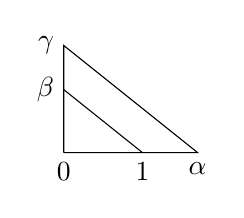
\begin{tikzpicture}[baseline=(Bs.base)]
		\node (Bs) at (0, 0.68) {};
		\draw (0,0) [below] node {$0$} -- (1.7, 0) [below] node {$\alpha$} -- (0, 1.36) [left] node {$\gamma$} -- (0,0);
		\draw (1,0) [below] node {$1$} -- (0, 0.8) [left] node {$\beta$};
	\end{tikzpicture}\]
	Dengan cara serupa, pembagian direduksi ke kasus pembagian bilangan positif. Diberikan $\gamma, \alpha > 0$, gambar di atas juga menunjukkan cara mengonstruksi $\beta = \gamma/\alpha$. 

	Karena kita telah mengetahui cara membagi dua argumen dari $\alpha \in \CC$, konstruksi akar kuadrat tereduksi ke kasus $\alpha > 0$. Perhatikan gambar berikut:
	\[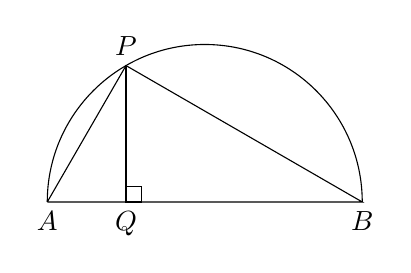
\begin{tikzpicture}[baseline=(Bs.base)]
		\node (Bs) at (90:1cm) {};
		\draw (0:2cm) arc [start angle=0, end angle=180, radius=2cm];
		\node (P) at (120:2cm) [above] {$P$};
		\draw (180:2cm) [below] node {$A$} -- (0:2cm) [below] node {$B$} -- (120:2cm) -- (180:2cm);
		\draw (120:2cm) -- (180:1cm) [below] node {$Q$};
		\draw (180:1cm) rectangle ++(0.2, 0.2);
	\end{tikzpicture} \quad |AQ|=1, \; |QB|=\alpha. \]
	Sifat kesebangunan memberikan $|PQ|=\sqrt{\alpha}$. Terakhir, konjugasi $\alpha \mapsto \bar{\alpha}$ tidak lain adalah pencerminan terhadap sumbu real.
\end{proof}
Lemma ini menyiratkan $\sqrt{-1} \in \text{Con}(\mathcal{S})$ dan
\[ z \in \text{Con}(\mathcal{S}) \iff \Re(z), \Im(z) \in \text{Con}(\mathcal{S}). \]

\begin{theorem}\label{prop:characterization-constructible}
	Diberikan subhimpunan $\{0, 1\} \subset \mathcal{S} \subset \CC$, berdasarkan pembahasan di atas kita boleh mengasumsikan bahwa $\mathcal{S}$ tertutup terhadap konjugasi kompleks. Tuliskan $\Q(\mathcal{S})$ untuk submedan yang dibangkitkannya. Maka suatu bilangan kompleks $z$ memenuhi $z \in \mathrm{Con}(\mathcal{S})$ jika dan hanya jika terdapat menara ekstensi medan
	\[ \Q(\mathcal{S}) = F_0 \subset F_1 \subset \cdots \subset F_n \subset \CC \]
	dengan $z \in F_n$, dan untuk setiap $0 \leq i < n$ berlaku $[F_{i+1} : F_i] = 2$. Khususnya, $z$ aljabar atas $\Q(\mathcal{S})$.
\end{theorem}
Dengan kata lain, kemampuan konstruksi dengan penggaris dan jangka tepat terdiri atas empat operasi aritmetika dan pengambilan akar kuadrat.
\begin{proof}
	Kita akan menggunakan sifat berikut: jika $E = F_m$ dan $E' = F'_n$ masing-masing merupakan suku terakhir suatu menara ekstensi kuadratik seperti di atas, maka kompositumnya $EE'$ juga demikian. Hal ini sangat mudah dibuktikan dengan rekursi pada $\max\{n,m\}$.

	Andaikan $z$ berada dalam $F_n$ seperti di atas. Karena di sini hanya terlibat medan berkarakteristik nol, setiap ekstensi kuadratik $F_{i+1}|F_i$ harus berbentuk $F_{i+1} = F_i(\sqrt{\alpha_i})$, dengan $\alpha_i \in F_i^\times$. Bersama Lemma \ref{prop:ruler-compass-aux}, segera diperoleh $z \in F_n \subset \text{Con}(\mathcal{S})$. Sebaliknya, ambil $z \in \text{Con}(\mathcal{S})$. Ingat definisi
	\[ \text{Con}(\mathcal{S}) = \bigcup_{k \geq 0} \mathcal{S}^{(k)}, \quad \mathcal{S}^0 = \mathcal{S}, \; \mathcal{S}^{(k+1)} = (\mathcal{S}^{(k)})'. \]
	Diberikan keluarga titik $z_j = x_j + y_j \sqrt{-1} \in \mathcal{S}^{(k)}$ ($j=1,\ldots, m$), dan andaikan semuanya berada dalam satu menara ekstensi kuadratik $\Q(\mathcal{S}) = F_0 \subset \cdots \subset F_n \subset \CC$; setelah mengambil kompositum, kita boleh mengasumsikan bahwa $F_n$ tertutup terhadap konjugasi kompleks. Persamaan garis dan lingkaran yang dikonstruksi dari $z_1, \ldots, z_m$ mempunyai koefisien yang merupakan polinomial dalam $x_j, y_j$, sehingga koefisien tersebut juga berada dalam $F_n$. Sekarang kita kaji semua kemungkinan titik perpotongannya, dengan mempertimbangkan bagian real dan imajiner secara terpisah:
	\begin{compactenum}[(a)]
		\item perpotongan garis dengan garis: sama dengan menyelesaikan sistem dua persamaan linear di atas $F_n$, sehingga $F_n$ tidak perlu diperluas;
		\item perpotongan garis dengan lingkaran: sama dengan menyelesaikan persamaan kuadratik berkoefisien dalam $F_n$, sehingga koordinat titik-titik potong berada dalam suatu ekstensi kuadratik dari $F_n$;
		\item perpotongan lingkaran dengan lingkaran: jika keduanya berpotongan di dua titik, pengurangan kedua persamaan lingkaran menghasilkan garis yang melalui titik-titik potong; jika keduanya bersinggungan di satu titik, diperoleh garis singgung persekutuan. Jadi kasus ini direduksi ke perpotongan garis dengan lingkaran.
	\end{compactenum}
	Dengan demikian, unsur-unsur $\mathcal{S}^{(k+1)}$ tetap termuat dalam suatu menara ekstensi kuadratik. Selesai.
\end{proof}

Sebagai akibatnya, $z \in \text{Con}(\mathcal{S})$ menyiratkan $[\Q(z, \mathcal{S}) : \Q(\mathcal{S})] \in 2^{\Z}$, tetapi kebalikannya secara umum tidak benar. Karakterisasi yang lebih lengkap dapat diberikan oleh teori Galois. Pertama, perhatikan bahwa karakterisasi $z$ dalam Teorema \ref{prop:characterization-constructible} sangat mirip dengan karakterisasi ekstensi yang dapat diselesaikan dengan radikal (Definisi \ref{def:radical-ext} dan Teorema \ref{prop:characterization-solvable-radicals}); perbedaannya hanya bahwa di sini $F_{i+1}$ diperoleh dengan menambahkan akar kuadrat pada $F_i$, sehingga syaratnya lebih ketat. Sifat ini juga dapat dikarakterisasi melalui teori grup sebagai berikut (diterapkan pada $F = \Q(\mathcal{S}) \subset \CC$).
\begin{theorem}\label{prop:characterization-constructible-2}
	Andaikan medan $F$ berkarakteristik $\neq 2$ dan $E|F$ merupakan ekstensi separabel hingga. Pernyataan-pernyataan berikut ekuivalen.
	\begin{enumerate}[(i)]
		\item Terdapat menara ekstensi medan kuadratik $F = E_0 \subset \cdots \subset E_n$ sedemikian sehingga $E \subset E_n$;
		\item Grup Galois dari penutup normal $E^\dagger|F$ merupakan grup-$2$ (ingat Definisi \ref{def:p-group}).
	\end{enumerate}
\end{theorem}
\begin{proof}
	Dengan mengulangi argumen dalam Teorema \ref{prop:characterization-solvable-radicals}, diketahui bahwa (i) ekuivalen dengan pernyataan bahwa $G := \Gal(E^\dagger|F)$ mempunyai deret komposisi $G = G_0 \supset \cdots \supset G_n = \{1\}$ yang memenuhi $G_i/G_{i+1} \simeq \Z/2\Z$. Khususnya, $G$ merupakan grup-$2$; karena $\text{char}(F) \neq 2$, kita tidak perlu lagi menggunakan teori Artin--Schreier atau menambahkan akar satuan, sehingga keadaan menjadi jauh lebih sederhana. Sebaliknya, Proposisi \ref{prop:p-group-nilpotent} menyiratkan bahwa setiap grup-$2$ solvabel, sehingga mempunyai deret komposisi semacam itu. Jadi (i) $\iff$ (ii).
\end{proof}

I.\ M.\ Isaacs \cite{Is85} menemukan suatu hasil terkait yang menarik: andaikan semua akar polinomial tak tereduksi $P \in \Q[X]$ adalah real. Misalkan salah satu akarnya, $\alpha$, dapat dinyatakan dengan radikal real. Ini berarti bahwa terdapat menara seperti dalam Definisi \ref{def:radical-ext}, yakni $\Q = E_0 \subset \cdots \subset E_n \ni \alpha$, tetapi dengan syarat $E_n \subset \CC$ dan akar yang ditambahkan pada setiap tahap $E_{i+1}|E_i$ semuanya real. Maka $\Gal(P)$ merupakan grup-$2$. Oleh karena itu, semua akar polinomial semacam ini dapat dikonstruksi dengan penggaris dan jangka.

Untuk kasus dengan syarat minimum $\mathcal{S} = \{0,1\}$, medan $\text{Con} := \text{Con}(\mathcal{S})$ terdiri atas semua bilangan kompleks yang dapat dikonstruksi dengan penggaris dan jangka dalam pengertian klasik. Sekarang kita dapat menangani tiga masalah konstruksi Yunani kuno yang pernah menguras pikiran begitu banyak pencinta matematika. Metode aljabar menunjukkan bahwa secara umum ketiganya tidak mempunyai penyelesaian di bawah pembatasan penggaris dan jangka.
\begin{description}
	\item[Duplikasi kubus] Diberikan suatu kubus beraturan dengan panjang rusuk $a$, bagaimana mengonstruksi kubus beraturan lain yang volumenya dua kali lipat? Di sini mengonstruksi kubus beraturan dipahami sebagai mengonstruksi panjang rusuknya. Masalah ini sama dengan, mulai dari $\mathcal{S} = \{0, 1, a\}$, mengonstruksi $b > 0$ sedemikian sehingga $b^3 = 2a^3$. Ambil $a=1$; maka $[\Q(2^{1/3}):\Q] = 3 \notin 2^{\Z}$ menunjukkan bahwa $b$ tidak dapat dikonstruksi dengan penggaris dan jangka.
	
	\item[Pengkuadratan lingkaran] Diberikan suatu lingkaran, dapatkah kita mengonstruksi dengan penggaris dan jangka sebuah persegi yang luasnya sama dengan luas lingkaran tersebut? Sekali lagi, masalah ini dapat dipahami sebagai konstruksi panjang sisi persegi, dan kita boleh mengambil jari-jari lingkaran sebagai satuan panjang $1$. Masalah ini lalu tereduksi menjadi konstruksi $\sqrt{\pi}$ dengan penggaris dan jangka. Jawaban atas masalah ini pada akhirnya bergantung pada transendensi $\pi$.

	\item[Triseksi sudut] Diberikan suatu sudut $\theta$ pada bidang, konstruksilah $\theta/3$ dengan penggaris dan jangka. Sebelumnya telah dikatakan bahwa mengonstruksi sudut $\theta$ sama dengan mengonstruksi $\omega := e^{i\theta}$ pada lingkaran satuan. Jadi masalah triseksi sudut sama dengan memulai dari $\mathcal{S} = \{0,1,\omega\}$ dan mengonstruksi $\eta := e^{i\theta/3}$, dengan $\eta^3 = \omega$. Untuk menunjukkan bahwa secara umum $\eta \notin \text{Con}(\mathcal{S})$, ambil $\theta := \pi/3$: jelas bahwa $\omega = \frac{1 + \sqrt{-3}}{2} \in \text{Con}$, sehingga masalahnya tereduksi menjadi pembuktian $\eta \notin \text{Con}(\mathcal{S}) = \text{Con}$. Andaikan sebaliknya; maka $\alpha := \Re(\eta) = \cos(\theta/3) \in \text{Con}$, tetapi rumus sudut rangkap tiga $\cos(3x) = 4 \cos^3 x - 3\cos x$ memberikan
	\[ 4\alpha^3 - 3\alpha - \cos\theta = 4\alpha^3 - 3\alpha - \frac{1}{2} = 0. \]
	Substitusi $\beta = 2\alpha$ memberikan $\beta^3 - 3\beta - 1 = 0$; mudah diperiksa bahwa $X^3 - 3X - 1 \in \Q[X]$ tidak mempunyai akar rasional, sehingga tak tereduksi. Oleh karena itu,
	\[ [\Q(\alpha):\Q] = [\Q(\beta) : \Q] = 3 \notin 2^{\Z} \]
	menunjukkan bahwa $\alpha \notin \text{Con}$, suatu kontradiksi.
\end{description}

Pembahasan triseksi sudut di atas membawa kita pada masalah konstruksi klasik lainnya: poligon beraturan bersisi $n$ manakah yang dapat dikonstruksi dengan penggaris dan jangka? Masalah ini dapat dirumuskan secara tepat sebagai berikut: bilangan $n \in \Z_{\geq 1}$ manakah yang memenuhi $\zeta_n := e^{\frac{2\pi i}{n}} \in \text{Con}$? (Silakan pembaca memikirkannya.)

Kita memerlukan konsep berikut: bilangan prima berbentuk $p = 2^{2^a} + 1$ disebut prima Fermat. Perhatikan bahwa $A \geq 1$ dan primalitas $2^A + 1$ menyiratkan $A = 2^a$. Memang, jika $d$ merupakan faktor prima ganjil dari $A$, matematika sekolah menengah memberikan $2^{A/d} + 1 \mid 2^A + 1$. Hingga tahun \the\year, satu-satunya prima Fermat yang diketahui adalah kasus $a=0,1,2,3,4$.\index{prima Fermat}

\begin{theorem}
	Suatu bilangan bulat positif $n$ memenuhi $\zeta_n \in \mathrm{Con}$ jika dan hanya jika $n$ berbentuk $2^a p_1 \cdots p_k$, dengan $p_1, \ldots, p_k$ prima Fermat yang berbeda-beda.
\end{theorem}
\begin{proof}
	Dengan menerapkan Teorema \ref{prop:characterization-constructible-2}, masalahnya tereduksi menjadi penentuan kapan grup Galois dari ekstensi siklotomik $\Q(\zeta_n)|\Q$, yang ditulis $G_n$, merupakan grup-$2$. Tuliskan $n = \prod_{p: \text{prima}} p^{n_p}$. Teorema sisa Cina bersama Teorema \ref{prop:cyclotomic-Galois} memberikan
	\[ G_n \simeq (\Z/n\Z)^\times \simeq \prod_{p: \text{prima}} (\Z/p^{n_p}\Z)^\times. \]
	Masalah semula tereduksi menjadi penentuan kapan $(\Z/p^m \Z)^\times$ merupakan grup-$2$. Karena grup ini mempunyai $p^m - p^{m-1} = p^{m-1}(p-1)$ unsur, sifat tersebut jelas berlaku ketika $p=2$. Ketika $p>2$, haruslah $m = 1$, dan dalam hal ini syarat perlu dan cukup agar diperoleh grup-$2$ ialah $p-1 = 2^A$, dengan $A \in \Z_{\geq 1}$. Ini tepat ekuivalen dengan pernyataan bahwa $p$ adalah prima Fermat.
\end{proof}

Untuk kasus khusus $n = 17$, konstruksi poligon beraturan bersisi 17 dengan penggaris dan jangka diberikan oleh Gauss pada tahun 1796; lihat \cite[\S 29]{Har00} untuk perinciannya. Pembuktian di atas juga mempunyai variasi sederhana berikut.
\begin{proposition}\label{prop:cos-rationality}
	Andaikan $\theta \in \Q\pi$. Maka $\cos\theta$ rasional jika dan hanya jika $\theta \in \left\{ \frac{\pi\Z}{2}, \frac{\pi\Z}{3} \right\}$.
\end{proposition}
Kasus yang bersesuaian mengikuti dari $\sin\theta = \cos(\frac{\pi}{2} - \theta)$; kasus $\sin\theta$ tidak akan diuraikan lagi.
\begin{proof}
	Cukup dibuktikan arah ``hanya jika''. Jika $a := \cos\theta \in \Q$, maka $e^{i\theta} = \cos\theta + i\sin\theta \in \Q(i \sqrt{1 - a^2})$. Tuliskan $\theta = \frac{2\pi m}{n}$, dengan $(n,m)=1$. Maka $\Q(\zeta_n) = \Q(e^{i\theta})$ menjadi ekstensi dari $\Q$ yang berderajat $\leq 2$. Dengan kembali menggunakan $\Gal(\Q(\zeta_n)|\Q) \simeq (\Z/n\Z)^\times$ dan meninjau faktorisasi prima dari $n$, diperoleh bahwa haruslah $n=2,3,4,6$; kasus-kasus ini dapat diperiksa satu per satu.
\end{proof}

% % % % % % % %
\begin{Exercises}
	\item Jika himpunan $X$ dilengkapi aksi kiri $\Gamma_F$, dan $\Stab_{\Gamma_F}(x)$, untuk setiap $x \in X$, merupakan subgrup terbuka dari $\Gamma_F$, maka $X$ disebut himpunan-$\Gamma_F$. Semua himpunan-$\Gamma_F$ hingga beserta pemetaan ekuivariannya membentuk kategori $\Gamma_F\dcate{Set}$. Di sisi lain, tuliskan $F\dcate{EtAlg}$ untuk kategori semua aljabar étale atas $F$ (Definisi \ref{def:etale-alg}), dengan homomorfisme aljabar-$F$ sebagai morfismenya. Buktikan bahwa $\Gamma_F\dcate{Set}^\text{op}$ ekuivalen dengan $F\dcate{EtAlg}$.
	\begin{hint}
		Definisikan funktor $\Theta: \Gamma_F\dcate{Set}^\text{op} \to F\dcate{EtAlg}$ sebagai berikut. Untuk $X$ yang diberikan, ambil $\Theta(X)$ sebagai subaljabar dari $(F^\text{sep})^X$ yang invarian di bawah $\Gamma_F$. Suatu pemetaan ekuivarian $f: Y \to X$ secara alami menginduksi $f^*: (F^\text{sep})^X \to (F^\text{sep})^Y$, dan selanjutnya menghasilkan $\Theta(f)$. Funktor kuasi-invers dapat diambil sebagai $\Hom_{F\dcate{EtAlg}}(-, F^\text{sep})$.
	\end{hint}
	\item Andaikan $p$ prima dan $\F_p \subset F$. Dengan mengikuti gagasan Lemma \ref{prop:pins-polynomial}, buktikan bahwa $X^p - X - a \in F[X]$ tak tereduksi jika dan hanya jika $a \notin \left\{b^p -b : b \in F\right\}$; buktikan pula bahwa dalam hal ini $F[X]/(X^p-X-a)$ merupakan ekstensi normal dari $F$.
	\item Andaikan $F$ suatu medan hingga berkarakteristik $p$, $n \geq 1$, dan $f_1, \ldots, f_m \in F[X_1, \ldots, X_n]$. Andaikan derajat totalnya memenuhi
		\[ \deg f_1 + \cdots + \deg f_m < n. \]
		\begin{compactenum}[(i)]
			\item Buktikan bahwa banyaknya penyelesaian $f_1 = \cdots = f_m = 0$ dalam $F^n$ adalah nol modulo p, yakni $\equiv 0 \pmod p$.
			\begin{hint}
				Misalkan $q := |F|$. Maka banyaknya penyelesaian $\bmod\; p$ kongruen dengan $\sum_{x \in F^n} \prod_{i=1}^m \left( 1 - f_i(x)^{q-1} \right)$; selain itu, $0 \leq k < q-1 \implies \sum_{a \in F} a^k = 0$.
			\end{hint}
			\item Simpulkan bahwa jika $(0, \ldots, 0)$ merupakan penyelesaian dari $f_1 = \cdots = f_m = 0$ (misalnya ketika $f_1, \ldots, f_m$ semuanya homogen), maka sistem persamaan tersebut harus mempunyai suatu penyelesaian yang tidak semuanya nol.
		\end{compactenum}
		Hasil ini disebut Teorema Chevalley--Warning. Hasil tersebut berkaitan dengan konsep berikut: medan $F$ disebut medan $C_1$ jika setiap polinomial homogen di atas $F$ dengan jumlah peubah lebih besar daripada derajat totalnya mempunyai penyelesaian $\neq (0, \ldots, 0)$. Jadi medan hingga merupakan medan $C_1$. C.-C. Tsen adalah orang pertama yang mempelajari medan $C_1$; sifat-sifat terkait berguna dalam kajian geometri aljabar aritmetika.
	\item Untuk setiap bilangan prima $p$ dan bilangan bulat positif $n$, buktikan
		\[ \Phi_{pn}(X) = \begin{cases} \Phi_n(X^p), & p \mid n \\ \dfrac{\Phi_n(X^p)}{\Phi_n(X)}, & p \nmid n. \end{cases} \]
	\item Buktikan bahwa untuk $n > 1$, suku konstan polinomial siklotomik $\Phi_n$ selalu $1$.
	\item Tetapkan $n \in \Z_{\geq 1}$ dan buktikan:
		\begin{enumerate}[(i)]
			\item Andaikan $p$ prima dan $p \nmid n$. Maka terdapat $a \in \Z$ sedemikian sehingga $\Phi_n(a) \equiv 0 \pmod p$ jika dan hanya jika $a \bmod p$, di dalam $(\Z/p\Z)^\times$, merupakan unsur berorde $n$; dalam hal ini $p \equiv 1 \pmod n$;
			\item Buktikan bahwa barisan $1 + n\Z_{\geq 1}$ memuat tak hingga banyak bilangan prima; ini merupakan kasus khusus Teorema Dirichlet.
		\end{enumerate}
	\item Untuk medan siklotomik $\Q(\zeta_n)$, buktikan $\Q(\zeta_n) \cap \R = \Q\left( \zeta_n + \zeta_n^{-1} \right)$. Hitung derajat ekstensinya atas $\Q$.
	\item Andaikan $p$ suatu prima ganjil. Buktikan bahwa $\Q(\zeta_p)$ memuat tepat satu submedan yang memenuhi $[E:\Q]=2$; submedan ini kita tulis $E$, dan $E \subset \R$ jika dan hanya jika $p \equiv 1 \pmod{4}$.
	\item Dengan menggunakan Teorema \ref{prop:indep-character-Artin} bersama Teorema \ref{prop:norm-trace-field}, buktikan kembali bahwa bentuk teras $(x,y) \mapsto \Tr_{E|F}(xy)$ dari suatu ekstensi separabel bersifat tak degenerat.
	\item Tentukan derajat $\Q(\sqrt{2},\sqrt{3})$ atas $\Q$, deskripsikan grup Galoisnya, dan berikan suatu basis normal.
	\item Buktikan bahwa suatu ekstensi Galois $E|F$ merupakan ekstensi abelian jika dan hanya jika setiap subekstensi hingga $M|F$ merupakan ekstensi abelian.
	\item Misalkan $D_1, \ldots, D_n$ bilangan bulat bebas kuadrat yang saling koprima. Tetapkan $L := \Q(\sqrt{D_1}, \ldots, \sqrt{D_n})$. Gunakan teori Kummer untuk membuktikan bahwa $L|\Q$ merupakan ekstensi Galois dan bahwa $\Gal(L|\Q)$ isomorfik dengan $(\Z/2\Z)^n$.
	\item Andaikan $P \in F[X]$ suatu polinomial berderajat $n \geq 1$ tanpa akar berulang, dengan akar-akar $\alpha_1, \ldots, \alpha_n \in F^\text{sep}$ dan medan pemisah $L$. Ingat diskriminan yang dibahas dalam Contoh \ref{eg:polynomial-discriminant}, yaitu $\delta := \prod_{i < j} (\alpha_i - \alpha_j)^2$; diskriminan ini merupakan polinomial dalam koefisien-koefisien $P$ dan tidak bergantung pada pengurutan akar. Andaikan $\mathrm{char}(F) \neq 2$.
		\begin{enumerate}[(i)]
			\item Buktikan bahwa $\Gal(L|F) \cap \mathfrak{A}_n = \Gal\left( L \;|\; F(\sqrt{\delta}) \right)$;
			\item Dalam kasus $n=2, 3$, tentukan rumus bagi $\delta(P)$ dan, berdasarkan rumus itu, berikan suatu metode untuk menentukan grup Galois sebuah polinomial kubik.
		\end{enumerate}
	\item Buktikan bahwa jika suatu subgrup $H \subset \mathfrak{S}_p$ memuat sebuah transposisi dan sebuah siklus-$p$ ($p$ prima), maka $H = \mathfrak{S}_p$.
	\item Andaikan polinomial tak tereduksi berderajat prima $p$, yakni $P \in \Q[X]$, mempunyai tepat $p-2$ akar real. Buktikan bahwa $\Gal(P) = \mathfrak{S}_p$. Berikan contoh konkret untuk $p=3$.
	\item Berikut ini kita mengkaji grup Galois dari polinomial kuartik $P = X^4 - a_1 X^3 + a_2 X^2 - a_3 X + a_4 \in F[X]$. Di sini $P$ diasumsikan tak tereduksi dan $\text{char}(F) \neq 2$, serta medan pemisahnya ditulis $L$.
		\begin{enumerate}[(i)]
			\item Buktikan bahwa setiap polinomial kuartik tak tereduksi di atas $F$ tidak mempunyai akar berulang, dan bahwa setiap polinomial kuartik tak tereduksi dapat dibawa ke bentuk di atas.
			\item Andaikan akar-akar $P$ dalam $L$ adalah $x_1, \ldots, x_4$. Definisikan
				\begin{align*}
					u & := x_1 x_2 + x_3 x_4, \\
					v & := x_1 x_3 + x_2 x_4, \\
					w & := x_1 x_4 + x_2 x_3.
				\end{align*}
				Dengan memandang $G := \Gal(L|F)$ sebagai subgrup dari $\mathfrak{S}_4$, buktikan bahwa $F(u,v,w) = L^{G \cap V}$, dengan
				\[ V := \{1, (1 2)(3 4), (1 3)(2 4), (1 4)(2 3) \} \lhd \mathfrak{S}_4, \quad V \simeq (\Z/2\Z)^2. \]
			\item Buktikan
				\[ Q := (X-u)(X-v)(X-w) = X^3 - a_2 X^2 + (a_1 a_3 - 4a_4) X - (a_1^2 a_4 + a_3^2 - 4a_2 a_4), \]
				dan bahwa $P, Q$ mempunyai diskriminan yang sama, yakni $\delta \in F^\times$; buktikan bahwa grup Galois dari $Q$ adalah $G/G \cap V$. Polinomial $Q$ lazim disebut resolven kubik dari $P$.
			\item Klasifikasikan subgrup-subgrup transitif dari $\mathfrak{S}_4$:
				\begin{inparaenum}[(a)]
					\item $\mathfrak{S}_4$,
					\item $\mathfrak{A}_4$,
					\item $V$,
					\item grup siklik berorde $4$ (semuanya saling konjugat),
					\item subgrup Sylow-$2$ $\simeq D_8$ (semuanya saling konjugat).
				\end{inparaenum}
			\item Susun tabel berikut:
				\[\begin{array}{c|c|c|c}
					\delta & Q \in F[X] & G & |G/G \cap V| \\ \hline\hline
					\notin F^{\times 2} & \text{tak tereduksi} & \mathfrak{S}_4 & 6 \\ \hline
					\in F^{\times 2} & \text{tak tereduksi} & \mathfrak{A}_4 & 3 \\ \hline
					\notin F^{\times 2} & \text{tereduksi} & D_8\; \text{atau}\; \Z/4\Z & 2 \\ \hline
					\in F^{\times 2} & \text{tereduksi} & V & 1
				\end{array}\]
		\end{enumerate}
	\item Lanjutkan dengan kasus pada soal sebelumnya ketika $\delta \notin F^{\times 2}$ dan $Q$ tereduksi. Dalam hal ini, medan pemisah $Q$ adalah $F(\sqrt{\delta})$. Jika $P$ tak tereduksi di atas $F(\sqrt{\delta})$, maka $G \simeq D_8$; jika tidak, $G \simeq \Z/4\Z$. Namun, ini bukan satu-satunya cara untuk membedakan kedua kasus tersebut.
	\item Lengkapi pembuktian Teorema \ref{prop:characterization-constructible-2}.
	\item Medan terurut adalah suatu medan $F$ yang dilengkapi sebuah subhimpunan $P \subset F$ (disebut kerucut positif) yang memenuhi
		\begin{compactitem}
			\item $x, y \in P \implies x+y, xy \in P$;
			\item $F = P \sqcup \{0\} \sqcup (-P)$.
		\end{compactitem}
		Buktikan bahwa
		\begin{compactenum}[(i)]
			\item definisi $x < y \iff y-x \in P$ menjadikan $(F, \leq)$ suatu himpunan terurut total;
			\item $0 < x < y \implies x^{-1} > y^{-1} > 0$
			\item $x < y$, $z > 0$ menyiratkan $xz < yz$;
			\item setiap jumlah kuadrat adalah $\geq 0$; khususnya, $\text{char}(F)=0$;
			\item $-1$ tidak dapat dinyatakan sebagai jumlah kuadrat. Berdasarkan hal ini, buktikan bahwa $\CC$ tidak dapat dilengkapi dengan struktur medan terurut.
		\end{compactenum}
	\item Andaikan medan terurut $F$ memenuhi syarat-syarat
		\begin{inparaenum}[(a)]
			\item $P = F^{\times\; 2}$ (jadi urutan sepenuhnya ditentukan oleh struktur medan $F$);
			\item setiap $Q \in F[X]$ berderajat ganjil mempunyai akar dalam $F$.
		\end{inparaenum}
		Buktikan berturut-turut bahwa
		\begin{compactenum}[(i)]
			\item satu-satunya ekstensi hingga berderajat ganjil dari $F$ adalah $F$ sendiri;
			\item $\left[ F(\sqrt{-1}) : F \right]=2$ dan setiap unsur dalam $F(\sqrt{-1})$ mempunyai akar kuadrat;
			\item dengan menerapkan Lemma \ref{prop:alg-closed-decomp}, simpulkan bahwa $F(\sqrt{-1})$ tertutup secara aljabar.
		\end{compactenum}
		\begin{hint}
			Andaikan $Q \in F[X]$ suatu polinomial tak tereduksi, dan misalkan $L|F$ medan pemisah dari $Q \cdot (X^2+1)$ serta $G := \Gal(L|F)$. Setiap subgrup Sylow-$2$, $H \subset G$, memberikan ekstensi berderajat ganjil $L^H | F$, sehingga $G$ merupakan grup-$2$. Jika subgrup $\Gal\left( L|F(\sqrt{-1})\right)$ tak trivial, maka Proposisi \ref{prop:p-group-nilpotent} bersama korespondensi Galois akan memberikan, di atas $F(\sqrt{-1})$ dan di dalam $L$, suatu ekstensi berderajat $2$, yang merupakan kontradiksi; jika $m=1$, haruslah $L=F(\sqrt{-1})$.
		\end{hint}

		Jelas bahwa $F=\R$ memenuhi syarat (a) dan (b), dan $\CC = \R(\sqrt{-1})$; jadi soal ini memberikan pembuktian lain bagi teorema dasar aljabar. Pembuktian-pembuktian lain yang lazim lebih bergantung pada alat-alat analisis seperti teori fungsi kompleks. Maksudnya di sini bukanlah menyingkirkan sebanyak mungkin unsur nonaljabar seolah-olah makin sedikit analisis selalu lebih baik, melainkan bahwa syarat-syarat ini benar-benar membantu menyingkap hakikat teorema dasar aljabar dan memperluasnya ke keadaan yang lebih umum. Medan $F$ yang memenuhi syarat (a) dan (b) disebut \emph{medan tertutup real}; lihat \cite[Bab 9]{Feng17}. Artin dan Schreier meletakkan dasar teori umum medan tertutup real; lihat \cite[Bab XI]{Lang02}. Barangkali hal yang lebih patut dicatat ialah bahwa medan tertutup real dapat dipandang sebagai pendahulu struktur $o$-minimal dalam teori model, yang mempunyai penerapan penting dalam geometri. \index{moxinglun}
\end{Exercises}
